% This is LLNCS.DOC the documentation file of
% the LaTeX2e class from Springer-Verlag
% for Lecture Notes in Computer Science, version 2.4
\documentclass{llncs}
\usepackage{llncsdoc}

\usepackage[T1]{fontenc}
\usepackage[latin1]{inputenc}
\usepackage[table, svgnames]{xcolor} 
\usepackage{color} 
\usepackage{url}
\usepackage{graphicx, array, blindtext}
\usepackage[tight,footnotesize]{subfigure}
\usepackage{mdframed}
\usepackage{latexsym}
\usepackage{boxedminipage}
\usepackage{ amssymb }
\usepackage[normalem]{ulem}
\usepackage{flushend}

\usepackage{ocgx}
\usepackage{listings}
\usepackage{tikz}
\usetikzlibrary{ocgx}

\usepackage{blindtext}
\usepackage{scrextend}
\usepackage{multirow}
\addtokomafont{labelinglabel}{\ttfamily}

\setlength\floatsep{1\baselineskip plus 3pt minus 2pt}
\setlength\textfloatsep{1\baselineskip plus 3pt minus 2pt}
\setlength\intextsep{1\baselineskip plus 3pt minus 2 pt}

\definecolor{dkgreen}{rgb}{0,0.6,0}
\definecolor{gray}{rgb}{0.5,0.5,0.5}
\definecolor{mauve}{rgb}{0.58,0,0.82}

\lstset{frame=tb,
	language=Java,
	aboveskip=3mm,
	belowskip=3mm,
	showstringspaces=false,
	columns=flexible,
	basicstyle={\small\ttfamily},
	numbers=left,
	numberstyle=\tiny\color{gray},
	keywordstyle=\color{blue},
	commentstyle=\color{dkgreen},
	stringstyle=\color{mauve},
	breaklines=true,
	breakatwhitespace=true,
	tabsize=3
}

%
%\lstdefinestyle{mystyle}{
%	basicstyle=\footnotesize,
%	breakatwhitespace=false,         
%	breaklines=true,                 
%	captionpos=b,                    
%	keepspaces=true,                 
%	numbers=left,                    
%	numbersep=5pt,                  
%	showspaces=false,                
%	showstringspaces=false,
%	showtabs=true,                  
%	tabsize=2
%}
%
%\lstset{style=mystyle} 
%
\begin{document}

\begin{center}

\LARGE \textbf{Why are program analysis tools difficult to understand?} \\
\Large A tool (mis)communication theory and adaptive approach for supporting developers during tool use \\[2.0em]

\end{center}

\begin{center}
	Brittany Johnson\\[1.0em]
	North Carolina State University \\
	bijohnso@ncsu.edu
	
\end{center}

\begin{abstract}
Program analysis tools are designed to aide any developer when developing software by automating the writing, analysis, and modification of source code. However, previous research suggest developers may not use these tools. When they do, gaps in developer knowledge and mismatches between what the developer knows and how the tool communicates prevent effective communication.
This thesis poses that program analysis tool use is a form of \textit{communication}, and the inability to interpret and resolve tool notifications is a result of miscommunication caused by \textit{knowledge gaps and mismatches}. Therefore, I propose tool design can be improved by approximating developer knowledge and experiences to adapt notifications to better align with individual developer preferences; this is inspired by \textit{constructivism} communication theory for improving communication by adapting to the audience.
I propose research that explores the feasibility, generalizability, and effectiveness of using models that can predict developer conceptual knowledge to improve tool communication by adapting notifications to the individual developers.
The contributions of this dissertation are: 1) a \textit{tool miscommunication theory} that explains the challenges developers encounter when interpreting tool notifications, 2) \textit{experiments and evaluations} that assess how valid and actionable the miscommunication theory is, and 3) a \textit{proof-of-concept tool}, called SmartBugs, that utilizes my proposed approaches for modeling and adapting tool notifications.
My research suggests that it is possible to create and use models of developer knowledge to improve tool and notification usability.
\end{abstract}

%\rule{\textwidth}{1pt}
%\begin{flushleft}
%\large\itshape
%\begin{tabular}{@{}l}
%{\Large\upshape\bfseries Springer}\\[8pt]
%Berlin\enspace Heidelberg\enspace New\kern0.1em York\\[5pt]
%Barcelona\enspace Budapest\enspace Hong\kern0.2em Kong\\[5pt]
%London\enspace Milan\enspace Paris\enspace\\[5pt]
%Santa\kern0.2em Clara\enspace Singapore\enspace Tokyo
%\end{tabular}
%\end{flushleft}


%
%{\tt svserv@vax.ntp.springer.de}\hfil first try the \verb|help|
%command.
%



%
%\newpage
%\tableofcontents
%\newpage
%

\section{My Thesis}


\fbox{
	\parbox{\textwidth}{Program analysis \emph{tool use} is a form of \emph{communication} and \emph{inability to interpret and resolve} notifications is a result of \emph{miscommunication} caused by \emph{knowledge gaps} and \emph{knowledge mismatches}; therefore we can improve tool design by applying \emph{constructivism} communication theory such that tools can \emph{approximate} individual developer's \emph{conceptual knowledge} to adapt notifications accordingly, leading to \emph{reduced time and context-switching} required for developers to interpret and resolve tool notifications.}
	}
% TODO make sure later it's obvious how (and why) will assess time and context-switching
%


\section{Research Significance}

\subsection*{Motivating Example}
% merge motivating examples from icse and fse papers into one big example (make sure detailed but say what I mean!)

\begin{figure} [ht]
	\centering
	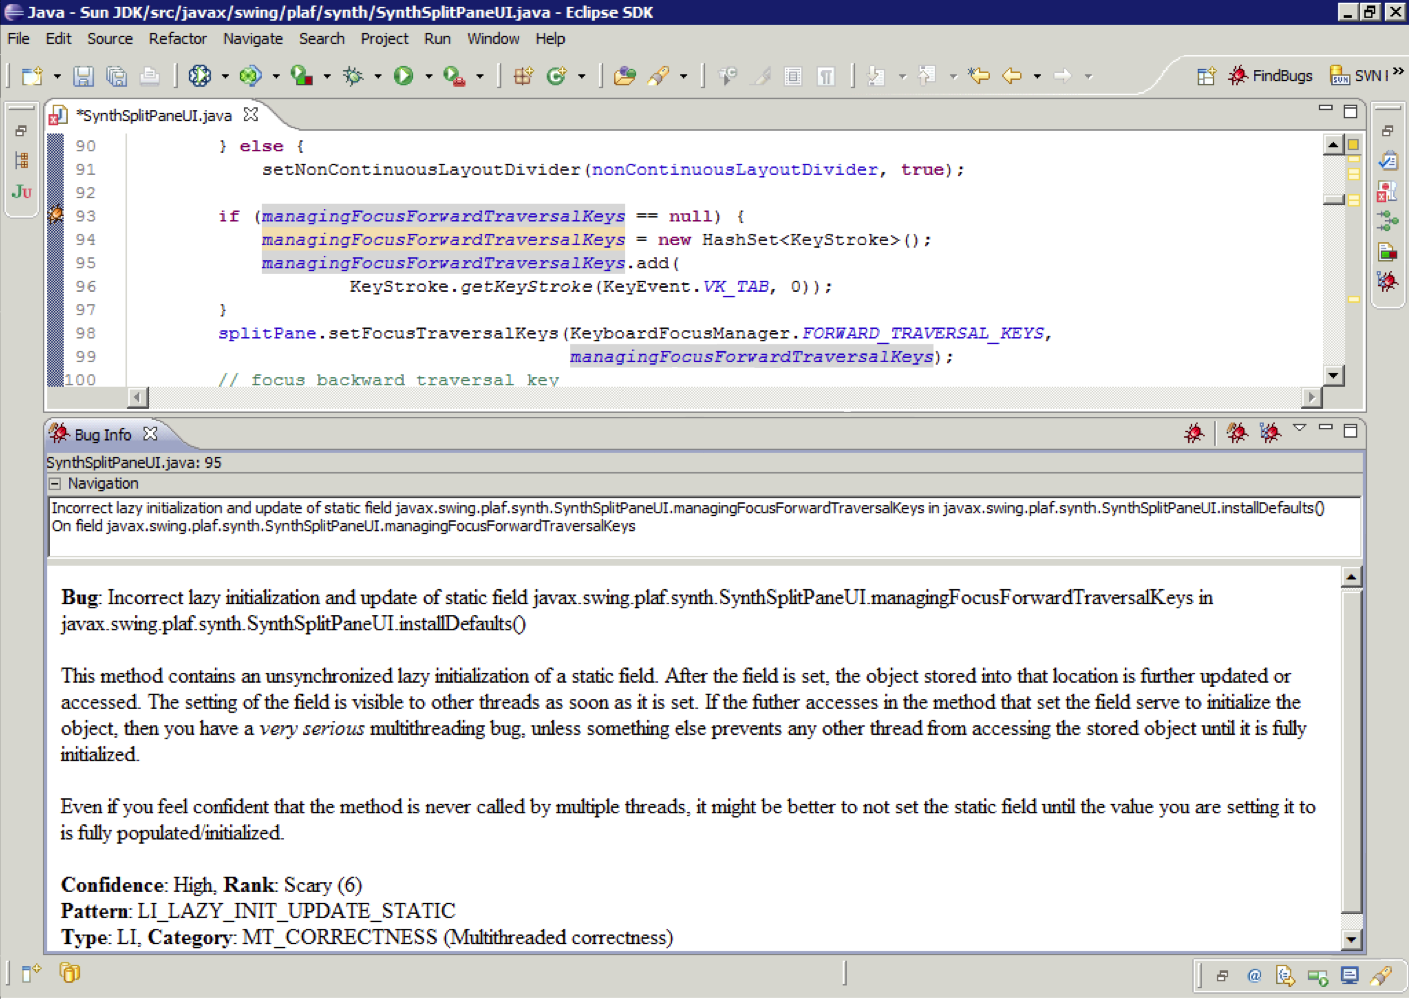
\includegraphics[width=\textwidth]{figs/eclipse.png}
	\caption{Findbugs notification in the Eclipse IDE concerning multi-threading.}
	\label{fig:eclipse}
\end{figure} 

Valerie is a software developer at a start-up company. She primarily writes Java code, though she did not learn to program in Java, and uses the Eclipse Integrated Development Environment (IDE). In her spare time, she builds her knowledge of Java programming concepts by contributing to open source software and using tools that provide feedback about the code she writes. While modifying code in the Sun JDK source code repository, she contributes code that results in the notification shown in Figure~\ref{fig:eclipse}. She has experience using FindBugs, so she is familiar with some of the ways FindBugs communicates. For example, she knows that an orange bug icon indicates a \textit{scary} bug and that by clicking the bug icon she can gain access to more information about the bug.

As she explores the information provided by FindBugs, she realizes that despite her experience with FindBugs, she is having difficulty determining how to resolve the notification. She first attempts to use what knowledge she does have regarding multi-threading, which she accrued from struggling with and resolving compiler synchronization warnings, to better understand the problem. 
% TODO not clear what "the problem" is - be specific
However, she is unfamiliar with the concept central to the notification in Figure~\ref{fig:eclipse} (lazy initialization). Though the notification tells her that the problem relates to multi-threading, she is unable to make a connection between her knowledge regarding multi-threading and the message FindBugs is attempting to communicate and therefore cannot resolve the notification without outside help. As done previously with compiler synchronization notifications, she toggles between the web and her IDE to understand and resolve the notification.

% TODO compiler synchronization notification??

\begin{figure} 
	\centering
	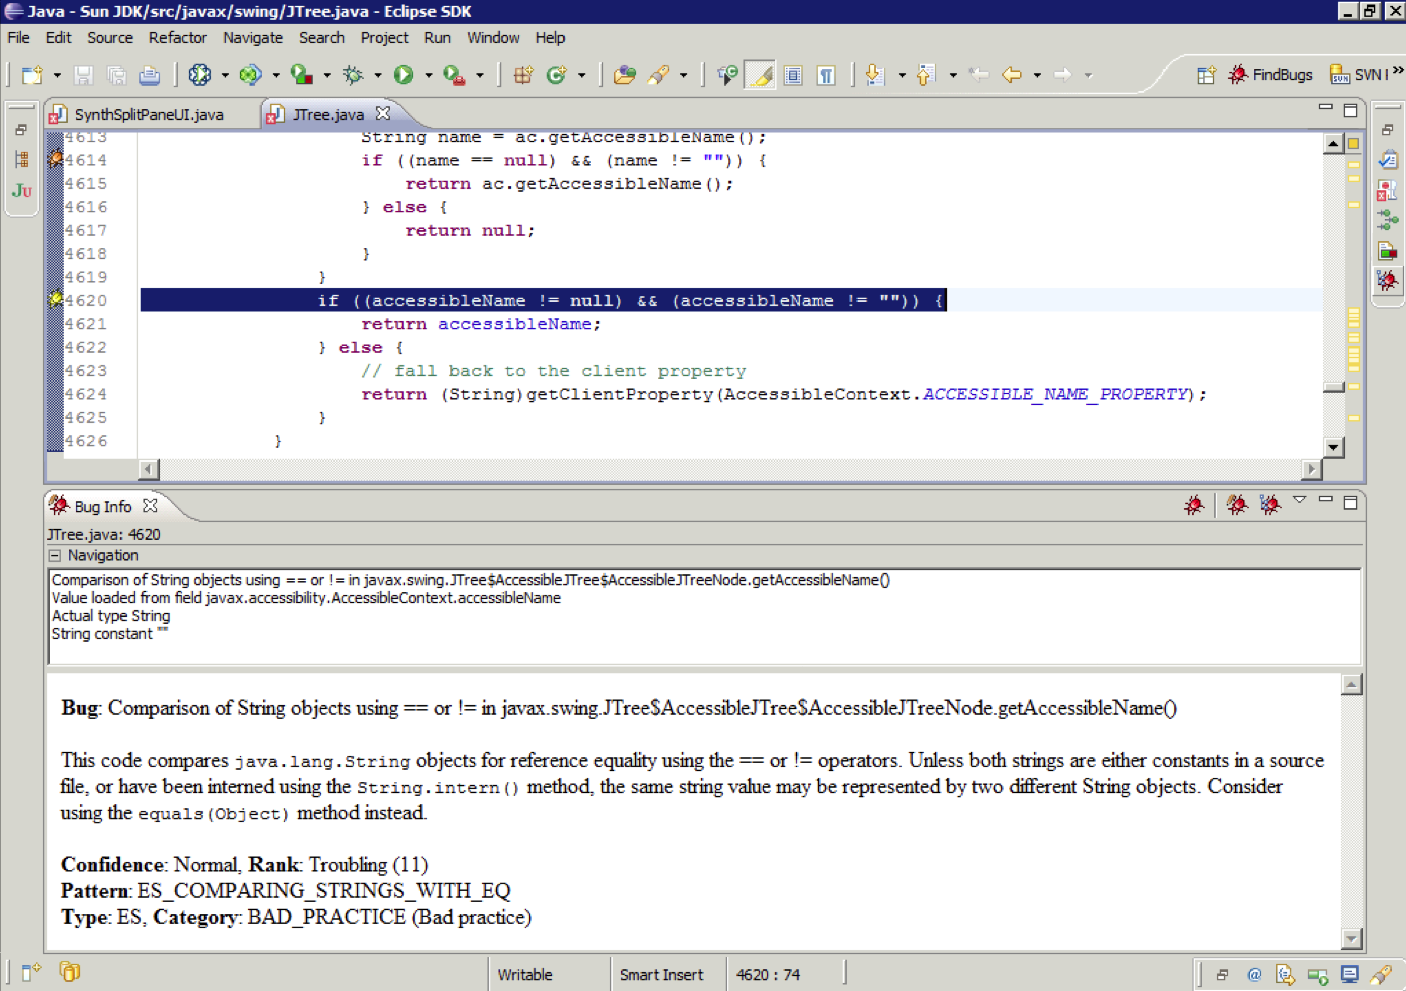
\includegraphics[width=\textwidth]{figs/eclipse-2.png}
	\caption{Findbugs notification in the Eclipse IDE on checking string equality.}
	\label{fig:eclipse2}
\end{figure}

Although Valerie's goal when using tools like FindBugs is to find and resolve defects, which requires the ability to interpret the notifications provided by the tools, a secondary goal is to learn more about Java programming concepts. She found, however, that some notifications are better at communicating problems while contributing to knowledge than others. For example, when first learning how to work with strings in Java, Valerie encountered the notification in Figure~\ref{fig:eclipse2}. The first time she encountered the problem she was able to understand and resolve the notification. Looking back, she realizes this was because the notification in Figure~\ref{fig:eclipse2} filled in gaps in her own knowledge of the concept by informing her \emph{why} what she was doing was wrong and \emph{how} she can fix it.

Because the tools Valerie uses have no notion of what she does and does not know, some notifications communicate in a way that she is able to understand the problem, while others are not, leading to  miscommunication. In the following sections, I will discuss research that explores challenges like those encountered by Valerie and motivate research for developing techniques, frameworks, and tools that mitigate these challenges.

\begin{figure} [ht]
	\centering
	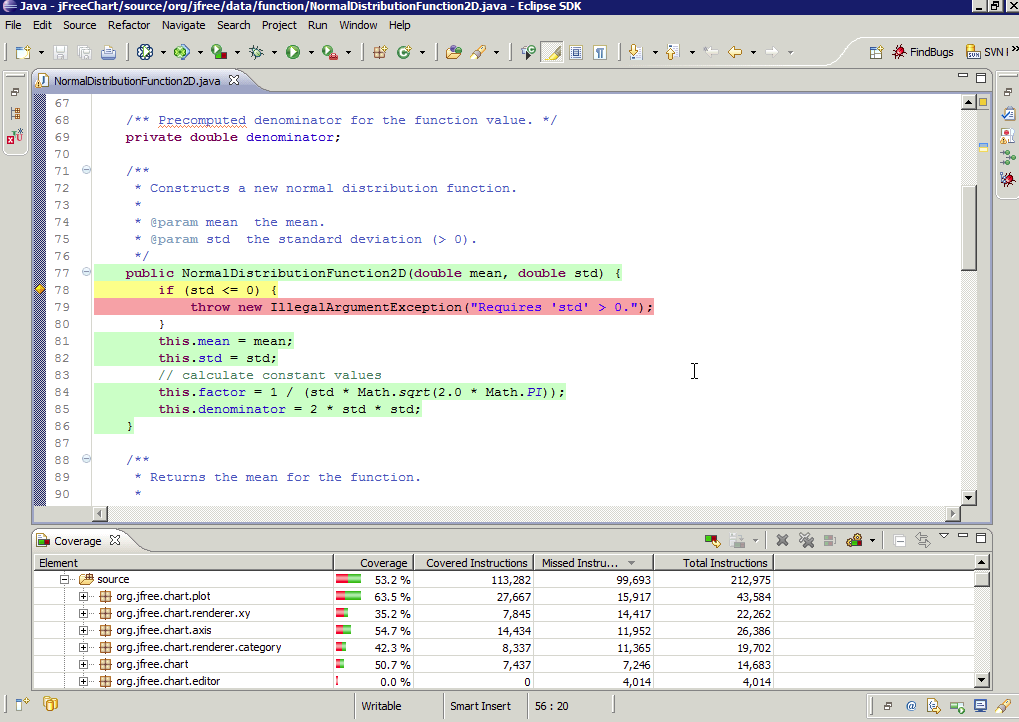
\includegraphics[width=\textwidth]{figs/eclemma.png}
	\caption{EclEmma notifications in the Eclipse IDE.}
	\label{fig:ecl}
\end{figure}

\subsection{What are program analysis tools?}
Program analysis tools are designed to aide developers when developing software by automating the writing, analysis, and modification of source code.
Often, program analysis is discussed as synonymous with static analysis~\cite{nielson2015principles}. 
For the purpose of my research, I define a program analysis tool as \emph{a recommendation system that performs program analysis, whether it be static or dynamic analysis, and provides information regarding the source code being analyzed}~\cite{robillard2014recommendation}.
Examples of program analysis tools include, but are not limited to, static code analyzers, code coverage tools, code smell detectors, and refactoring tools~\cite{adolph2011using,Murphy-Hill:2010:Ambient,ge2012reconciling}.
Program analysis tools can be used in integrated development environments (IDEs) as well in most text editors that can be used for programming, such as Vim~\footnote{http://www.vim.org/} or Emacs~\footnote{https://www.gnu.org/software/emacs/}. 
In the following sections, I will define and discuss static analysis and dynamic analysis tools separately; the reader should note that although I discuss static and dynamic analysis separately, it is not uncommon to find program analysis tools that combine static and dynamic analysis~\cite{ernst2003static}.                                                

\subsubsection{Static Analysis Tools.}

Static analysis tools are designed to aide developers when developing software by statically analyzing source code, pre-runtime, and providing the developer with feedback about the state of their code~\cite{ernst2003static}.
Typically, static analysis works by examining the current state of the program, predicting how the program may react in that state at runtime, and reporting any information they deem necessary to the developer. Static analyses are often more conservative than dynamic analyses; this is to reduce the potential for false positives, as in most cases static analysis cannot say with 100\% certainty what will happen during run-time. 
Examples of static analysis tools include defect detectors, such as FindBugs, compilers, code smell detectors, and refactoring tools.
% TODO talk about what static analysis can do/find to motivate further

Let's use the example of FindBugs,\footnote{http://findbugs.sourceforge.net/factSheet.html} an open source static analysis tool, to better understand how static analysis tools work. FindBugs statically analyzes code to report potential defects. FindBugs determines the potential for defects using \emph{bug patterns}. Bug patterns are code idioms that map to errors, found in Java \emph{bytecode}. Bytecode, in Java, represents the compiled Java class files. Because FindBugs analyzes code without executing it, there is a heightened risk for \emph{false positives}. False positives are defects detected that will never manifest during run-time. When FindBugs finds a potential defect, it alerts the developer using notifications that provide information regarding the defect. I will discuss tool notifications in more detail in Section~\ref{subsec:comm}.


\subsubsection{Dynamic Analysis Tools.}

Dynamic analysis tools are designed to aide developers when developing software by analyzing source code during run-time and providing the developer with feedback about runtime behavior~\cite{ernst2003static}.
Dynamic analysis works by executing the program and then making observations about program execution; because dynamic analysis runs the code, it is typically more precise than static analysis. Though dynamic analysis can produce more precise results in a similar amount of time as static analysis, dynamic analysis execution is less likely to generalize to future executions since it is based on a set of inputs that can, and probably will, change for each execution.
Examples of dynamic analysis tools include testing, code coverage, and profiling tools.

Let's use the example of Cobertura,\footnote{http://cobertura.github.io/cobertura/} an open source dynamic code coverage tool, to better understand how dynamic analysis tools work. Cobertura executes source code using JUnit test cases and reports to the user what parts of the code got covered and what parts did not. Because Cobertura executes the source code, it can communicate precisely regarding the flow of the program during run-time. A static code coverage tool could speculate how much of a code base would be covered based on test cases, and possibly even a set of inputs; however, it would require more effort and be more likely to produce false positives than a dynamic code coverage tool. On the down side, the test suites a developer writes may not be characteristic of all possible executions of the program, thereby lowering the generalizability of dynamic analyses.

\subsection{How do tools communicate?}\label{subsec:comm}

One common thread between program analysis tools like FindBugs and Cobertura is that they use \emph{notifications} to communicate with the developer. Figure~\ref{fig:ecl} and Figure~\ref{fig:eclipse} provide examples of tool notifications. 
A notification, when speaking in terms of program analysis tools, is typically a combination of visuals and text used to communicate a message to its user; for program analysis tools, the user is the developer.
Text editors like Vim and Emacs rarely include any visual components, however, because text editors are a simpler versions of IDEs, research on notifications in IDEs are more likely to backwards apply to text editors than vice versa. 
Therefore, I focus my research on notifications inside IDEs.

Notifications across tools vary; some provide lots of text (like FindBugs) with few visual aides, some use primarily visual means of communications (like Cobertura). Notifications can also have different goals, which may influence how developers design notifications. For example, the goal of a notification from Coverity~\footnote{http://www.coverity.com/}, another static analysis tool, is to explain a potential defect in the developer's source code and, ideally, help the developer make a decision about the defect (i.e. whether and how to resolve). Because Coverity's goal is to explain, we expect to see textual notifications that provide that explanation.
The goal of code coverage notifications is to statically show dynamic program behavior and help the developer determine the effectiveness of her test suite. EclEmma, another code coverage tool, uses colors applied directly to the source code to communicate as opposed to text. Though EclEmma also uses text to communicate code coverage (i.e. \texttt{1 of 2 branches missed} on a partially covered \texttt{if} statement), this does not allow the developer to scan the program for areas in most need of attention. Therefore, EclEmma uses other visuals, such as the bar visuals in the Coverage View (Figure~\ref{fig:ecl}) to show coverage on a given package or class.
 % TODO talk about how different parts of notification communicate for each tool; make sure it ties back to goals (defects and test coverage)!

The list of tools and notifications tools use can go on and on, but for the purposes of my research, the general definition I will use for a notification is \emph{a combination of visual and textual interfaces used by a program analysis tool to communicate information to developers about their source code.} Notifications can vary regarding what information and how much detail they provide, however, there are commonalities across tool notifications that informed this definition, which I will discuss next.

\subsection{What are the typical components of a tool notification?}
% based on robilliard book
One reason I talk about program analysis tools as a type of recommendation system is because they provide information to developers completing software engineering tasks~\cite{robillard2014recommendation}. 
Another reason is that program analysis tools use the same strategies defined by Robillard as typical of recommendation systems: 1) strategies for getting the user's attention and 2) descriptive interfaces.
Program analysis tools use these strategies when communicating with developers via notifications.

There are a variety of ways that a tool can get the attention of its user~\cite{robillard2014recommendation}. Program analysis tool notifications get the attention of developers in their IDEs in one or more of the following ways: icons, dashboards, pop-ups, affordance overlays, annotations, or email notifications.
Once the tool has the developer's attention, program analysis tool notifications provide descriptive interfaces that convey information about a developer's source code. 
Information is conveyed using some combination of textual, visual, and sometimes transformative descriptions.

Some tools, like FindBugs and most IDE compilers, use icons to get developers' attention. Using the same icons, developers can access more information either by hovering over or clicking the icon. Although the icons are visual, most of the description provided by these tools is textual. As stated previously, these kinds of notifications are most common with static analysis tools as they typically need to be more descriptive. However, dynamic analysis tools like Veracode~\footnote{http://www.veracode.com/products/dynamic-analysis-dast/dynamic-analysis}, which communicate about defects similar to the ones reported by FindBugs and Coverity, also use icons and text descriptions to pass along information to the developer.

\begin{figure}
	\centering
	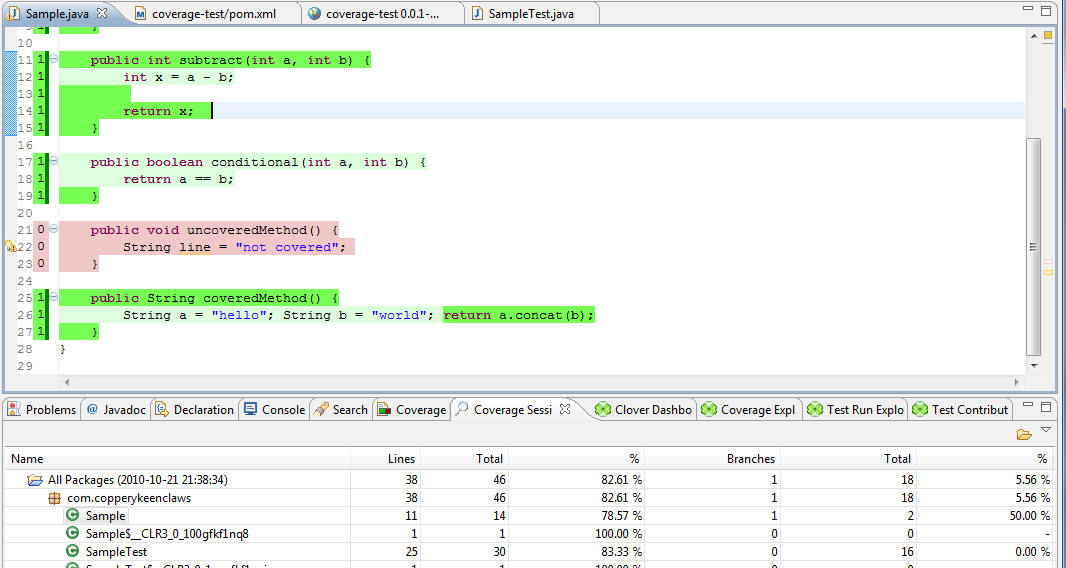
\includegraphics[width=3in]{figs/cobertura.png}
	\caption{Notifications provided by Cobertura regarding code coverage.}
	\label{fig:cobertura}
\end{figure}

\begin{figure}
	\centering
	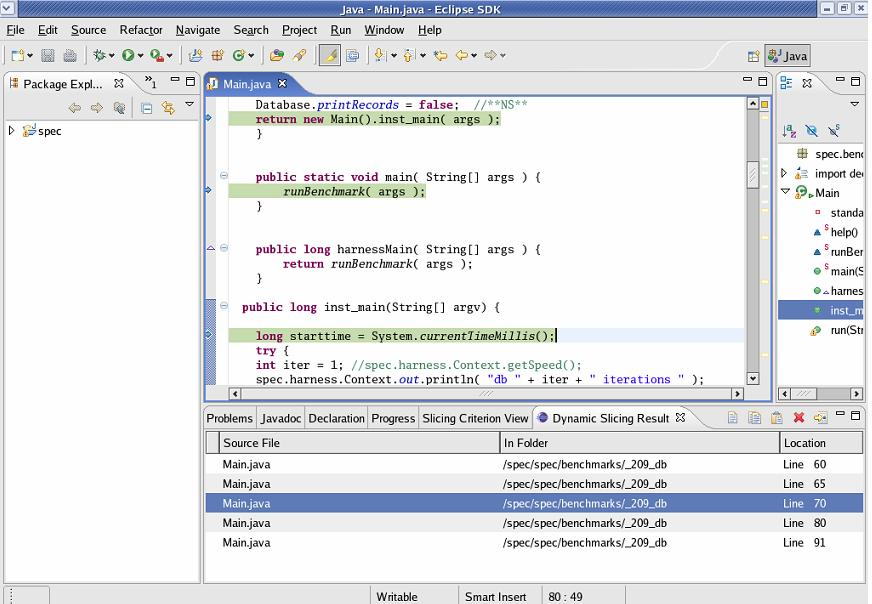
\includegraphics[width=3in]{figs/jslice.jpg}
	\caption{Notifications provided by JSlice regarding a dynamic slice of the program.}
	\label{fig:jslice}
\end{figure}


Some tools use affordance overlays or annotations to both get the attention of the developer and for the descriptive interface. For example, Cobertura and JSlice~\footnote{http://jslice.sourceforge.net/} use affordance overlays in the form of source code highlighting, as shown in Figure~\ref{fig:cobertura} and Figure~\ref{fig:jslice}, to alert the developer of and communicate about dynamic behavior. Coverity Dynamic Analyzer~\footnote{http://www.coverity.com/library/pdf/Coverity-Dynamic-Analysis.pdf}, which is similar to Veracode, uses annotations, such as the one in Figure~\ref{fig:coverity} in the editor to communicate about defects in the code.

\begin{figure}
	\centering
	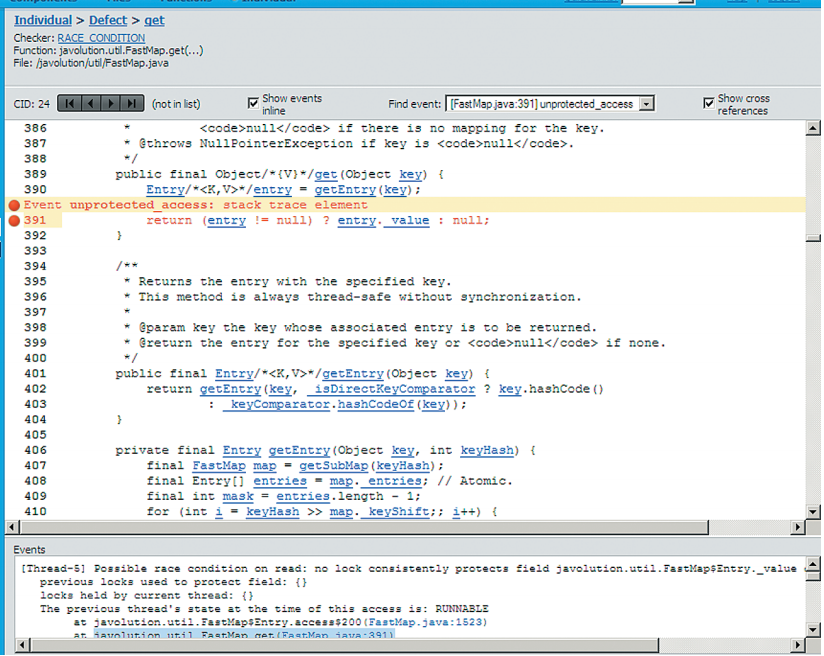
\includegraphics[width=3in]{figs/coverity-dynamic.png}
	\caption{A notification provided by Coverity regarding a race condition.}
	\label{fig:coverity}
\end{figure}

A small subset of tools use dashboards, such as the one shown to the right in Figure~\ref{fig:stench}. StenchBlossom, a code smell detection tool gets and maintains a developer's attention using an ambient dashboard~\cite{Murphy-Hill:2010:Ambient}. At anytime the developer is interested in the information being provided by the tool, the developer can use options in the dashboard to explore code smells present in their code base. The description is visual, using color overlays that map to each type of code smell. 

\begin{figure}
	\centering
	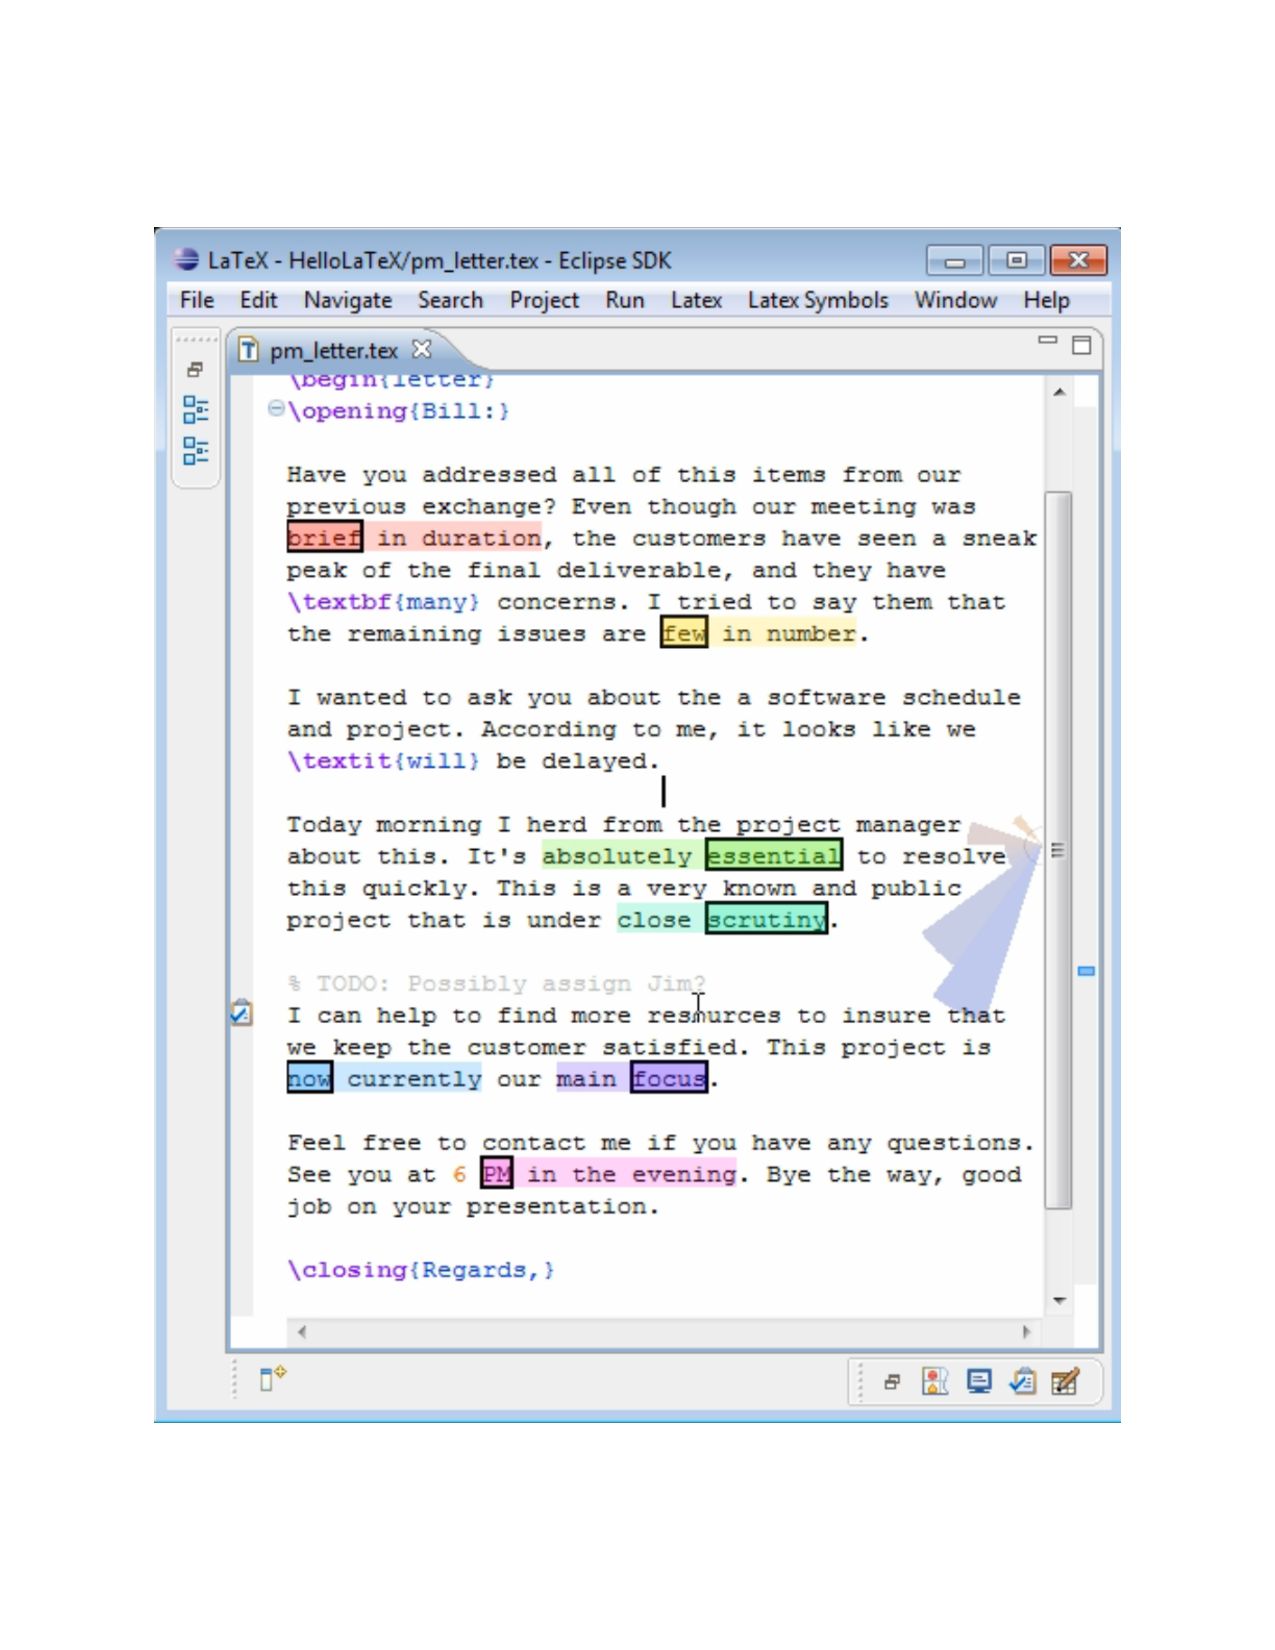
\includegraphics[width=3in]{figs/stenchblossom.pdf}
	\caption{Notifications provided by StenchBlossom regarding code smells.}
	\label{fig:stench}
\end{figure}

\begin{figure}
	\centering
	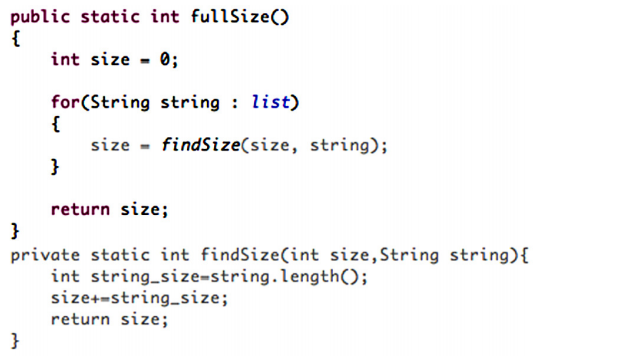
\includegraphics[width=3in]{figs/witchdoctor.png}
	\caption{A notification provided by WitchDoctor regarding a refactoring that's taking place.}
	\label{fig:witch}
\end{figure}

Finally, an even smaller subset of program analysis tools provide transformative descriptive interfaces. Transformative interfaces provide the developer with some idea of how the suggestion being made would affect the task at hand. For example, WitchDoctor, a refactoring tool, detects refactorings and then makes the developer aware of their refactoring by offering to complete the refactoring for the developer. To inform this process, WitchDoctor provides information regarding the assumed refactoring by showing the developer within their text editor what will happen if the refactoring is applied, as shown in Figure~\ref{fig:witch}.


% types of descriptions (text and visual)
% goals of information provided (??)

\subsection{What do tool notifications communicate about?}

% communicate about the state of with source code
The goal of program analysis tool notifications is to communicate some information to the developer about her source code about the task at hand.
The source code a developers writes is a runnable manifestation of programming-oriented and human-oriented concepts~\cite{van2004concepts,biggerstaff1994program}. 
At the lowest, most fundamental level, are \emph{programming-oriented concepts}, which relate to how the source code maps to programming language concepts. For simplicity, I will refer to these concepts simply as programming concepts.
Programming concepts can be as simple as the means for storing and passing data, such as variables, or as complex as the means for structuring data, such as generics~\cite{jazayeri1997programming}.
At a more abstract level, \emph{human-oriented concepts} relate to the high level requirement of the source code, such as ``acquire target'' or ``complete transaction''.

Typically a given notification is associated with only one human-oriented concept, though not all tools communicate about human-oriented concepts. For example, refactoring tools do not communicate about requirements such as ``acquire target.'' These kinds of tools typically focus on programming concepts; refactoring tools attempt to communicate about programming concepts such as variables and modules.
On the flip side, there can be more than one notification pertaining to a one human-oriented concept and one notification can communicate about more than one programming concept. 


Consider, for example, the following source code:

\begin{lstlisting}
	private BufferedWriter bufferedLogWriter = null;
	private static LogWriter theWriter = null;
	private Service loggingService = null;
	private boolean demoMode = true;
	
	public void writeLog(String eventString) {
	
		if (isDemoMode()) {
			//DebugLogger.log("Sending: " + eventString);
			Sender.send(eventString);
		} else {
			try {
				openLogForWriting();
				if (bufferedLogWriter != null) {
					bufferedLogWriter.append(eventString);
					bufferedLogWriter.append("\n");
					bufferedLogWriter.flush();
					bufferedLogWriter.close();
				}
				DebugLogger.log("Writing: " + eventString);
	
			} catch (IOException e) {
				DebugLogger.log("Couldn't write to " + bufferedLogWriter);
				e.printStackTrace();
			}
		}
	}
\end{lstlisting}

The requirement, or human-oriented concept, at play is ``write to log file''. 
A notification attached to this code is telling the developer something about the code she wrote to ``write to log file''.
There are multiple programming concepts at play, which aligns with the types of notifications the developer could get. 
In the process of writing this code, the developer could get a notification regarding any number of programming concepts (buffered streams, exception handling); for example, tools like FindBugs, Sonar, and IntelliJ's built-in static analyzers notify developers when they have opened a stream (\texttt{BufferedWriter} in the above example) and there is a possibility the stream that is writing to the file is not closed.
A developer may also get a notification regarding exception handling. Here, the developer has written code to catch an \texttt{IOException} if it occurs. However, if she did not implement code to deal with the potential for an \texttt{IOException} she would get a compiler notification communicating the need to do so.


% TODO later, should note that focusing on programming oriented concepts because those generalize and are foundational to developing the abstractions that are human oriented concepts (biggerstaff)


\subsection{Are developers able to interpret tool notifications?}
Despite the possibility provided by program analysis tools for exploration and improvement of source code, research has found that developers often to not use program analysis tools~\cite{Ayewah:2008:FindBugs,ge2012reconciling}.
Though research has explored tool usage, there was no research that explored the reasons developers have for using the tools they do use and not using the tools they do not use~\cite{Bessey:2010:Coverity,Khoo:2008:PathProjection}.
To answer the question \emph{why do developers not use program analysis tools}, I conducted interactive interviews with 20 professional developers to better understand why they do not use static analysis tools, one common type of program analysis tool, to find bugs when writing code~\cite{johnson2013don}.

Based on the data from these interviews, some of the reasons developers do not frequently use static analysis tools are \textbf{Lack of collaborative support}, \textbf{Seemingly unorganized tool output}, \textbf{Poor support for customizations}, and \textbf{Difficult to interpret notifications}. 
Three out of four findings regarding tool use pertain to the notifications tools use and how tools present information to the developer.
Discovering that tool notifications are one of the reasons developers do not use program analysis tools is useful, however, not actionable. The next piece of information needed to make these findings actionable is to discover what about tool notifications make it difficult for developers to interpret them.

\section{A Tool Miscommunication Theory}\label{sec:theory}
%session study (fse)\\
% TODO need something relevant to cross-tool!
To answer the question \emph{why do developers encounter challenges when interpreting program analysis tool notifications?}, I observed 26 developers with varying backgrounds while they used three different program analysis tools: Eclipse Java compiler, FindBugs, and EclEmma. I presented participants with and asked them to interpret notifications from each of the three tools. 
To identify challenges, we examined tool use through the lens of communication theory~\cite{bowman1987modeling}.
Building on an existing model of (mis)communication~\cite{mustajoki2008modelling}, we identified 12 kinds of challenges developers encounter when interpreting tool notifications.

Based on the challenges participants encountered when interpreting tool notifications, I proposed a tool miscommunication theory that can be used to inform the design of program analysis tools.
Experts in qualitative research suggest that rather than presenting a set of disparate findings, qualitative researchers should instead produce an explanatory theory, a ``skeleton or framework that explains why things happen''~\cite{corbin2014basics}. While explicitly putting forward theories is rare in software engineering~\cite{hannay2007systematic}, one example is Lawrance and colleagues' theory of how programmers navigate code during debugging~\cite{lawrance2013programmers}. In the same way that Lawrance and colleagues' build on 
information foraging theory~\cite{pirolli1999information}, my theory builds on communication theory~\cite{bowman1987modeling}.
I summarize my theory as:

\begin{quotation}
	\noindent
	\emph{The challenges developers encounter when interpreting program analysis tool notifications are caused by gaps and mismatches between developer knowledge and how notifications communicate information.}
\end{quotation}

Because research has suggested experience matters when understanding vulnerabilities, and that experiences affect knowledge, I speak about knowledge here and throughout as the culmination of experiences~\cite{johnson1989mental,argote2011organizational,baca2009static}.
Using that definition, a \emph{knowledge gap} occurs when there is a gap between what the developer knows and how the tool communicates; a \emph{knowledge mismatch} occurs when what the developer knows and expects from the tool does not match the notification the tool uses.

Remember Valerie? Though she is a hypothetical developer, the challenges she faced are not hypothetical. Valerie experienced challenges caused by both knowledge gaps (no knowledge regarding lazy initialization) and knowledge mismatches (expecting an explicit connection to synchronization). Based on this theory, I hypothesize that if it was possible for tools to be aware of what developers know and do not know, tools can improve communication by adapting its notifications to the developer.

\section{A Proposed Approach for Modeling Developer Knowledge}
%modeling approach (vlhcc)
In order to adapt tool notifications to a given developer's knowledge, there needs to be some notion of how much the developer knows about the concepts in the notification. For the remainder of this document, I use concept to mean programming concepts. I chose to focus on programming concepts because existing research conducted by Smith and colleagues suggests understanding programming concepts affects developers' ability to resolve notifications~\cite{smith2015questions}. Borrowing from education research and using developer experiences as a concrete representation of knowledge, I evaluate the possibility to learn and approximately predict developer knowledge of programming concepts.

\subsection{Using Concept Inventories to Assess Concept Knowledge}
% TODO read through and revise as needed! 
To create any kind of model, I need a dependent variable and one or more independent variables that could be used to predict the value of the dependent variable. Since I want to build models that predict knowledge, my dependent variable has to be some measure of developer concept knowledge.
Borrowing from existing computer science education research, I developed concept inventories for knowledge assessment. 


Traditionally, concept inventories are used to  assess conceptual knowledge and identify misconceptions; in Computer Science, the target audience is typically CS1 students~\cite{tew2010developing,kaczmarczyk2010identifying}. 
I need to assess knowledge with a wide range of developers outside of academia, therefore I could not borrow directly from research that creates concept inventories for novice academic programming concept knowledge assessment~\cite{tew2010assessing}. I combined existing concept inventory research with examinations using revised Bloom's Taxonomy~\cite{tew2010developing,nelson1967testing,scott2003bloom}. By using Bloom's Taxonomy to inform question creation, I increased assurance that my questions exhaustively assess understanding~\cite{scott2003bloom}. 
The final process I have developed for creating general programming concept inventories is as follows:

\vspace{0.5em}
\noindent\textbf{Define Conceptual Content for Test Specification.} A test specification is a way of formally outlining what will be on the test without having to write the questions~\cite{tew2010developing}. Once you have decided on the programming concept of interest, use language tutorials surrounding that concept to define conceptual content. This process should be exhaustive; the sub-concepts covered for a given concept in any tutorial found should be included in the test specification.

\vspace{0.5em}

\noindent\textbf{Build Bank of Test Questions.} This step is where Bloom's Taxonomy becomes important. Without using Bloom's Taxonomy, I could create a group of questions that potentially assess the same level of understanding. To assess different levels of understanding, each question should map to at least one level of Bloom's Taxonomy. If possible, it is helpful to compare the kinds of questions asked to assess each level of Bloom's Taxonomy with the questions in the bank to be used.
It is also more effective if each level of Bloom's Taxonomy is represented in the bank of questions.

\vspace*{0.5em}

\noindent\textbf{Pilot Questions.} Once you have a bank of questions, the next step is to pilot the questions on the target audience. The goal of this pilot is to note the range in scores to inform validation, which is the next step. If all the scores are really high, or really low, this might suggest an assessment that is too difficult or too easy~\cite{nelson1967testing}, which would require revisiting and revising the test bank.

\vspace*{0.5em}

\noindent \textbf{Establish Validity and Reliability.} Validation of an assessment tool can be done in a variety of ways. The most common form of validation is item analysis~\cite{gorsuch1997exploratory}. The purpose of item analysis is to determine how effective your test, and the items on it, for knowledge assessment. This includes determining at a more granular level which questions may be too hard, too easy, or unfair. 
An example of an unfair question is a question where more than one response is a reasonable response, making it more difficult to determine the best response, even for an easy question.

%I discuss the process that led to this final set of steps when I related study in Section~\ref{subsec:s3}.

\subsection{Using Public Git Repositories to Predict Concept Knowledge}
As a developer, many experiences are focused on writing and modifying source code; writing software is also perhaps one of the most concrete actions that can be labeled as an experience for a developer. Therefore \emph{concept-specific source code} can be used to determine independent variables for concept knowledge models. I define concept-specific code as code that maps to a given programming concept; an example of multi-threading-specific code is \texttt{synchronized(variable)}, where the developer has written code that synchronizes variables for multi-threaded execution.

To accurately create models, we need to be able to attribute code changes to a specific developer; their contributions are coupled with concept inventory scores to create and evaluate the models. Analyzing static code can detect the presence of concept-specific code, such as synchronization or generics usage. However, it can not tell me who contributed that code, which is important when trying to build models that can accurately predict individual knowledge. 
Using version control can automate and ease the process of assigning code contributions to a given developer. 
Version control is also useful for determining how recently a developer has made concept-specific code contributions, which may be an important factor when using experience as a proxy for knowledge~\cite{johnson2015bespoke}. % TODO cite vlhcc here if accepted!
Given the ability to model concept knowledge, the next step is to assess the use of these models to determine appropriate information to give a developer in a given notification.


\section{An Argument for Knowledge-Based Notifications}
% bespoke paper (focused on notifications - fse)
% TODO proof-read and integrate with the rest of paper
Based on the ability to model and predict developer concept knowledege, I propose that program analysis tools could improve communication with developers by aligning notifications with the experience and knowledge of the developer using the tool.
For example, FindBugs provides the following notification:

\vspace*{-1ex}
\begin{quotation}
	\noindent \small{
		This call to a generic collection method passes an argument while compile type Object where a specific type from the generic type parameters is expected. Thus, neither the standard Java type system nor static analysis can provide useful information on whether the object being passed as a parameter is of an appropriate type.}
\end{quotation}
\vspace*{-1ex}

\noindent
A developer who is less familiar with concepts related to generic types might find this notification difficult to understand. 
In contrast, a developer who is very familiar with these concepts might find this notification too verbose or even distracting.

A tool that has access to models that can predict what a developer knows about programming concepts could adapt the notification to the developer looking at it.
To continue the above example, if a developer knows little about the concept of generic types, the message would be more verbose, perhaps providing links to relevant on-line material or example solutions.
If a developer knows all the relevant concepts well, the notification could instead simply say ``unchecked generic type,'' and point her to where in the code the generic type parameters are expected.

The code that the developer has written is a useful source of data for hints about a developer's knowledge of a concept.
For the generic type notification, this includes usage of generics where a generic type parameter is specified and usage of generic objects.
Another source would be notifications she has already resolved; if the developer has resolved notifications of the same kind or notifications that involve the same concepts, the developer likely has some knowledge of the underlying concepts.

In the above sections, I have outlined the significance and idea behind my proposed research; next I will outline the studies, experiments, and evaluations I have completed and will complete for my dissertation.

\section{Experiments \& Evaluations}\label{sec:eval}
% TODO think about RQs for each
% why don't study (completed)
This section outlines the research I have completed and will complete for my dissertation. For each study, I provide an abbreviated name in brackets ([]) to facilitate discussion about projects and results in later sections.

\subsection{Why don't developers use program analysis tools? [Reasons]\protect\footnote{Publication: Johnson, B., Song, Y., Murphy-Hill, E., \& Bowdidge, R. (2013, May). Why don't software developers use static analysis tools to find bugs?. In Software Engineering (ICSE), 2013 35th International Conference on (pp. 672-681). IEEE.}}\label{subsec:s1}

\subsubsection{Study rationale.} Static analysis tools provide a means for analyzing code without having to run
the code, helping ensure higher quality software throughout the development process. There are a variety of ways to perform automatic static
analyses~\cite{Gegick:2007:AutomatedAnalysis}, including at the developer's request, continuously while creating the software in a development
environment, and just before the software is committed to a version control system. The tool may allow the developer to configure what kinds of bugs it
finds, and sometimes even define new bug patterns. Static analysis tools use well-defined programming rules to find defects early in the development process, when they
are cheap to fix~\cite{Ayewah:2008:FindBugs}. For example, there are static analysis tools that can alert developers to synchronization issues which can
lead to unsafe thread interactions. Developers have been able to eliminate many defects that were previously overlooked at large companies~\cite{Ayewah:2010:GFF} using the warnings produced
by static analysis tools. 
Despite the benefits of using static analysis tools to find bugs, consistent usage of these tools is not very frequent~\cite{Ayewah:2008:FindBugs}. 
There have been studies to investigate ways of improving static analysis tools. However, none explore \emph{why} they do or do not use existing tools~\cite{Bessey:2010:Coverity,Khoo:2008:PathProjection}. 

\subsubsection{Research questions.}
\begin{labeling}{questions}
	\item [RQ1] What reasons do developers have for using or not using static analysis tools to find bugs?
	\item [RQ2] How well do current static analysis tools fit into the workflows of developers? 
	\item [RQ3] What improvements do developers want to see made to static analysis tools?
\end{labeling}

\subsubsection{Methodology.}
To answer my research questions, I used semi-structured interviews. Each semi-structured interview consisted of three parts: \textit{Question and  Short Response}, \textit{Interactive Interview}, and \textit{Participatory Design}. Once completed, I transcribed and coded each interview. Here I briefly describe each part of the interview and my coding process.
Research materials can be found on-line.\footnote{http://www4.ncsu.edu/~bijohnso/ffsat.html}

\vspace{0.5em}
\noindent\textit{Question and Short Response.} During the Question and Short Response portion of the interview, we asked developers questions related to their general usage, understanding, and opinion of static analysis tools in order to answer RQ1. Questions asked can be found on-line with other research materials.

\vspace{0.5em}
\noindent\textit{Interactive Interview.}
The goal behind an interactive interview was observe developers actually using a static analysis tool; for the study, the tool was FindBugs. I provided 6 open source projects in Java, such as log4j~\cite{log4j} and Ant~\cite{ANT}, and asked each participant to run FindBugs on one of them. I chose FindBugs because it is one of the most popular and mature static analysis tools for Eclipse. I used information obtained during this portion of the interview to answer RQ1 and RQ2. I asked participants to explain what they are doing out loud~\cite{Lewis:1982:ThinkAloudProtocol} so I could get a better understanding of their workflow and thought process as they used the tool. I define a workflow as the steps a developer takes when writing, inspecting and modifying code.

\vspace{0.5em}
\noindent\textit{Participatory Design.}
I used the last part of the interview to solicit participant design suggestions for improving static analysis tools. I utilized a concept called participatory design~\cite{Spinuzzi:2005:Participatory}, which involves
getting stakeholders (in this case, developers) involved in the design process by allowing them to show what they want instead of saying it. To promote creativity, I gave each participant a blank sheet of paper and asked them to show me what they wanted their tool to look like and how it should work~\cite{Johnson:2012:PreFFSAT}. It was not mandatory for participants to draw something, but 6 of them did. Figure~\ref{fig:drawing} shows an example drawing from one participant. The other participants gave verbal descriptions of tool features they desired.

\begin{figure} [h]
	\centering
	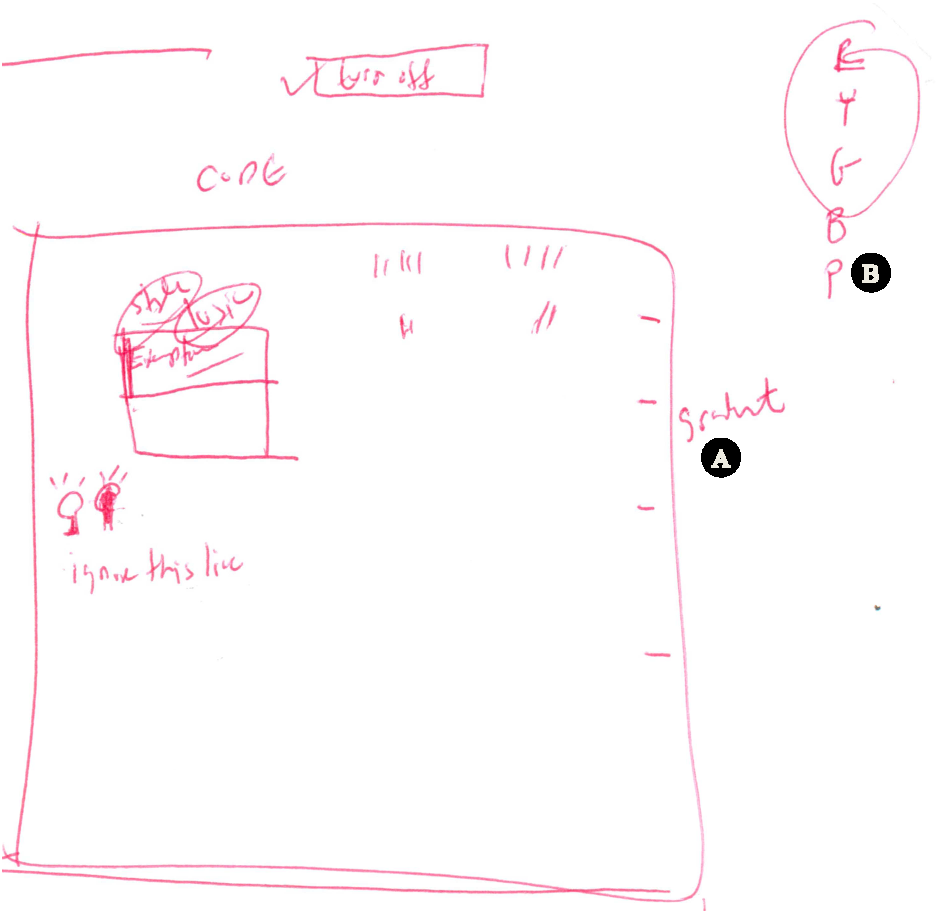
\includegraphics[width=4in]{figs/participatory.pdf}
	\caption{One participant's participatory design drawing; (A) shows where Matt wants the gradient colors and (B) shows the way his current tool represents severity.}
	\label{fig:drawing}
\end{figure}

\vspace{0.5em}
\noindent\textit{Coding Interview Responses.}
After completing the interviews, I manually transcribed each interview. Then, I \textit{coded} the final transcripts. Coding is a process that is meant to make referencing transcriptions quicker and
easier~\cite{Gordon:1998:Coding}. I used Gordon's basic steps to code the interviews. Before coding an interview, ``coding categories'' needed to be defined. For example, one coding category was \textbf{Workflows}. 
Some coding categories emerged after reading the transcripts.
The final set of coding categories are as follows: 

\begin{description}
	\item[Tool Output] -- Anything related to the output produced by the tool (for example, false positives). 
	\item[User Input/Customizability] -- Anything about the customizability of the static analysis tools (for example, modifying rule sets). 
	\item[Supporting Teamwork] -- Anything about using static analysis tools in a team or collaborative setting. 
	\item[Result Understandability] -- Anything about the ability or inability to understand or interpret the results produced by a static analysis tool.
	\item[Workflows] -- Anything related to the steps a developer takes when writing, inspecting and modifying their software (for example, tool integration).
	\item[Tool Design] -- Proposed tool design ideas from participants.
\end{description}

To ease indexing in the transcripts, I used color to identify each coding category.
The last step was to check the reliability of the codings. Once I finished coding the interviews, I passed the transcripts off to four other researchers to look over. If they found any discrepancies, we discussed and resolved them as a group. This included items that could fall into more than one category; in this situation, either a new, more specific, category or a ``sub-category'' was created for the item. The purpose of the categories are to organize the data in a relevant and useful manner; they are not meant to directly correlate with the research questions.

\subsubsection{Participants.} I conducted this study with 20 participants. I recruited participants using a recruitment flyer sent out to industry contacts. Sixteen participants were professional developers at a large company and 4 were graduate students at NC State University with previous industry experience. Participant development experience ranged from 3 to 25 years.

\subsubsection{Results.} As I discuss my findings, I use parentheses after each theme to denote how many participants discussed topics in each theme. 
Participants discussed the following as reasons they \emph{do} use static analysis tools (\textbf{RQ1}): 
\begin{description}
	\item[Automation (5)] Static analysis tools automate bug finding, and sometimes bug solving. Developers use static analysis tools to save time and effort when maintaining their code.
	\item[Availability (3)] Some development environments, such as IntelliJ IDEA~\footnote{https://www.jetbrains.com/idea/}, come with built-in static analysis tools. Developers also use static analysis tools because they are already installed and available in their IDEs, requiring little effort on their parts to at least adopt the tool.
	\item[Customizability (3)] Some tools allow its users to customize anything from the appearance of the tool's output to the type of output that is presented. Developer use static analysis tools when they are able to make desired customizations.
\end{description}

On the flip side, participants discussed the following reasons they \emph{do not} use static analysis tools (\textbf{RQ1}): 
\begin{description}
		\item [Collaboration (9)] Software development is inherently collaborative; some participants noted that tools they use and have used do not provide support for collaborative code improvement efforts.
		\item [Tool Output (14)] Findings prior to this study found that tools can produce large volumes of notifications, many of which end up being false positives~\cite{Ayewah:2010:GFF,Shen:2011:EFindBugs}; I found that this output can be overwhelming as presented by current tools. Participants noted that more intuitive and user-friendly output could help minimize the effects of dealing with these characteristics of tool output.
		\item [Customizability (17)] Developers want to configure their tools to present output how and when they want; currently tools do not effectively support the customizations developers want to make. If they do support customizations, the support is minimal and often time-consuming to use.
		\item [Result Understandability (19)] In order to effectively use static analysis tools, developers need to be able to interpret the notifications provided. Currently, many of the tools participants use provide cryptic notifications that lead to challenges for them when attempting to interpret the message.
\end{description}

I also explored the ability for existing tools to integrate with developer workflows (\textbf{RQ2}). Based on feedback from 19 participants, the following are workflow integration concerns:
\begin{description}
	\item[IDEs vs. Text Editors] Developers have preferences regarding how they want their tool integrated into their work environment. For example, some developers use IDEs so it is ideal if the tool can integrate with their IDE. Some developers do not use IDEs, so they would prefer compiler-level integration provided by some tools, like Clang\footnote{http://clang.llvm.org/docs/ClangTools.html}.
	\item[Tight Integration] Another important factor is how tight the integration is; some participants used IntelliJ as an example of an IDE with good tool and workflow integration due to the fact that the static analysis is built-in. This includes the tool running without having to be explicitly invoked by the developer.
	\item [Fast Feedback] Participants noted that another important part of workflow integration is the ability to give fast feedback; the sooner the tool can alert the developer to a problem in their code, the better the tool integrates into their workflow.
\end{description}

Finally, participants elaborated a number of ideas for how current static analysis tools could improve (\textbf{RQ3}). 
The majority of design suggestions fell into one of two categories: \textbf{Quick Fix Design} and \textbf{Warning Notification and Manipulation Design}.
\begin{description}
	\item[Quick Fix Design (10)] Quick fixes automatically resolve defects by applying a fix to the developer's code on her behalf. Suggestions participants had for improving this feature include providing fix previews through diffs and providing dialog boxes for walking through and toggling between fixes. 
	\item [Warning Notification and Manipulation Design (20)] All participants had suggestions for improving how and when notifications are presented to them. Suggestions for notifications include providing fast, discrete feedback and allowing developer to make and apply on-the-fly judgements, such as temporary suppression, to a given notification. 
\end{description}

%Other suggestions made by participants throughout their sessions include having ``plastic'' editors that fold and expand to show and hide information, visual output (i.e. pie-style diagram of project and bugs in it), and using a heat map to show where the most critical bugs in a project are. One interesting suggestion was to use gradient colors instead of multiple different colors to represent defect severity. Figure~\ref{fig:drawing} shows one of the drawings completed by a participant during participatory design; his suggestions focused on effective use of color for error representation, as have previous studies~\cite{Oberg:1992:Gradients,Murphy-Hill:2010:Ambient}.


\subsection{Why do developers have difficulty interpreting tool notifications? [Challenges]\protect\footnote{Publication: Johnson, B., Pandita, R., Smith, J., Ford, D., Elder, S., Murphy-Hill, E., Heckman, S., Sadowski, C., What We Have Here is a Failure to Communicate! A Cross Tool Study on Program Analysis Tool Notifications. FSE 2016 (in submission)}}\label{subsec:s2}
% session study (completed)
\subsubsection{Study rationale.} Program analysis tools, such as static analysis tools, refactoring tools, and code smell detectors, can ease manual and sometimes tedious software development tasks by automatically analyzing and modifying source code~\cite{adolph2011using,Murphy-Hill:2010:Ambient}. 
Output from these tools, such as warnings and errors, come in the form of textual or visual notifications that vary from tool to tool.
In previous interviews, 19 professional developers reported not using static analysis tools, one type of program analysis tool, because notifications can be difficult to interpret~\cite{johnson2013don}. The goal of this study was to understand what makes it challenging for developers to interpret program analysis tool notifications. To identify challenges, I examined tool use through the lens of communication theory~\cite{bowman1987modeling}. 

\subsubsection{Research question.}
Using Hannay and colleagues' guidelines~\cite{hannay2007systematic}, I framed my research question as \emph{why} rather than \emph{what} to support building a theory that explains the challenges developers encounter, yielding the following research question:

\begin{labeling}{questions}
	\item [RQ1] Why do developers encounter challenges when interpreting program analysis tool notifications? 
\end{labeling}



\subsubsection{Methodology.} To answer my research question, I observed participants while using three different program analysis tools.

\vspace{0.5em}
\noindent\textit{Program Analysis Tools Investigated.}
My research currently focuses on tools that can be used in the Eclipse Integrated Development Environment (IDE)~\cite{EclipseIDE}. I chose Eclipse because it is one of the most widely used IDEs~\cite{Goth:2005:Beware}, making it easier to recruit qualified participants, and because it is compatible with a variety of tools. I selected FindBugs, the Eclipse Java Compiler, and EclEmma as mature, popular tools. FindBugs is a static analysis tool for detecting potential defects in Java source code. The Eclipse Java compiler alerts developers of warnings and errors related to compilation and potential run-time problems. EclEmma is a Java code coverage tool. Examples of notifications used by these tools are shown in Figure~\ref{fig:N4} (FindBugs), Figure~\ref{fig:notificationCOMP} (compiler), and Figure~\ref{fig:notificationECL}.

\begin{figure} 
	
	\subfigcapskip = 1pt
	\subfigure[Source Code]{
		\fcolorbox{lightgray}{white}{\parbox{\dimexpr\linewidth-2\fboxsep-2\fboxrule}{
				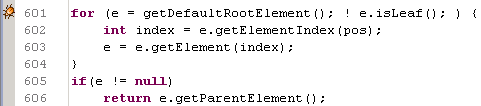
\includegraphics[width =3.3in] {figs/N4(no_tooltip)}
			}}
			\label{fig:N4code}
		}
		
		%The space between the figure and the caption
		\subfigcapskip = 1pt
		\subfigure[Short Description]{
			%From http://tex.stackexchange.com/questions/120530/wrapping-text-inside-framebox
			%\framebox (or fcolorbox) makes the box around the text.  The \parbox allows for wrapping
			%The \dimexpr stuff makes it fit in the column.  You don't need manual
			\fcolorbox{lightgray}{white}{\parbox{\dimexpr\linewidth-2\fboxsep-2\fboxrule}{
					{\scalebox{.8}{Nullcheck of e at line 605 of value previously dereferenced in \texttt{javax.-}} \\
						\scalebox{.8}{\texttt{swing.text.DefaultStyledDocument.getParagraphElement(int)} } \\
					}
					
					\label{fig:N4tooltip}
				}}
			}
			\subfigcapskip = 1pt
			\subfigure[Full Description]{
				\fcolorbox{lightgray}{white}{\parbox{\dimexpr\linewidth-2\fboxsep-2\fboxrule}{
						
						{\scalebox{.8}{A value is checked here to see whether it is null, but this value can't} \\
							\scalebox{.8}{be null because it was previously dereferenced and if it were null a null} \\ 
							\scalebox{.8}{pointer exception would have occurred at the earlier dereference.} \\ 
							\scalebox{.8}{Essentially, this code and the previous dereference disagree as to} \\ 
							\scalebox{.8}{whether this value is allowed to be	null. Either the check is redundant} \\ 
							\scalebox{.8}{or the previous dereference is erroneous.} 
						}
						
						\label{fig:N4full}
					}}
				}
				\caption{A notification of a previous null check from FindBugs (FB4).}
				\label{fig:N4}
			\end{figure}


\begin{figure} 
	\subfigcapskip = 1pt
	\centering
	\subfigure[Source Code]{
		\fcolorbox{lightgray}{white}{\parbox{\dimexpr\linewidth-2\fboxsep-2\fboxrule}{
				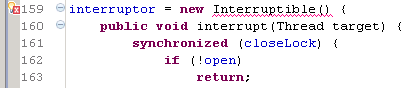
\includegraphics[width=2.6in]{figs/comp-notification}
				\label{Compcode}
			}}}
			\subfigcapskip = 1pt
			\subfigure[Text Description]{
				\fcolorbox{lightgray}{white}{\parbox{\dimexpr\linewidth-2\fboxsep-2\fboxrule}{
						
						{\scalebox{.8}{The type \texttt{new AbstractInterrruptibleChannelInterruptible()} } \\
							\scalebox{.8}{must implement the inherited abstract method \texttt{new AbstractInterr-}} \\ 
							\scalebox{.8}{\texttt{uptibleChannel.Interruptible.interrupt()}}
						}
						
						\label{Comptext}
					}} }
					
					\caption{An Eclipse compiler notification about unimplemented methods (CMP5).}
					\label{fig:notificationCOMP} 
				\end{figure}

\begin{figure} 
	\subfigcapskip = 1pt
	\centering
	\subfigure [Source Code with Highlighting]{ 
		\fcolorbox{lightgray}{white}{\parbox{\dimexpr\linewidth-2\fboxsep-2\fboxrule}{
				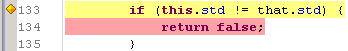
\includegraphics[width=2.3in]{figs/EclExample}
				\label{ECLcode}
			}}}
			\subfigcapskip = 1pt
			\subfigure[Text Description]{
				\fcolorbox{lightgray}{white}{\parbox{\dimexpr\linewidth-2\fboxsep-2\fboxrule}{
						\centering
						{\small ~~~1 of 2 branches missed~~~ }
						\label{Ecltext}
					}}
				}
				
				\caption{An EclEmma notification about partial branch coverage (ECL3).}
				\label{fig:notificationECL}
			\end{figure} 

\vspace{0.5em}
\noindent\textit{Study Protocol.} 
Participants engaged with each tool I investigated during sessions that each lasted approximately one hour. Each session consisted of seventeen tasks. 
For each task, I presented participants with and asked them to interpret one or more notifications from each tool.
I disallowed the use of a web browser to isolate the challenges developers encounter to the notifications used by the tools and to exclude challenges caused by outside tools.
During many tasks, and at least once for every participant, participants discussed or completed notification resolution. I did not require them to do so, since it would be unfair to ask them to resolve a notification if they did not understand it.
As participants explained the notifications, I asked follow-up questions as necessary. 


For each task, I chose notifications to represent the types of notifications developers may encounter when programming.
For FindBugs and the Eclipse compiler, I chose notifications that appeared frequently in the Sun JDK project. I chose EclEmma notifications from JFreeChart to exercise a range of its coverage scenarios. Because EclEmma's documentation does not specify the range of notifications it uses, I manually went through JFreeChart's codebase after running the tool and took note of each new coverage scenario encountered. I then included an example of each coverage scenario in the EclEmma tasks.

\begin{figure} 
	\subfigcapskip = 1pt
	\centering
	\subfigure[Source Code]{
		\fcolorbox{lightgray}{white}{\parbox{\dimexpr\linewidth-2\fboxsep-2\fboxrule}{
				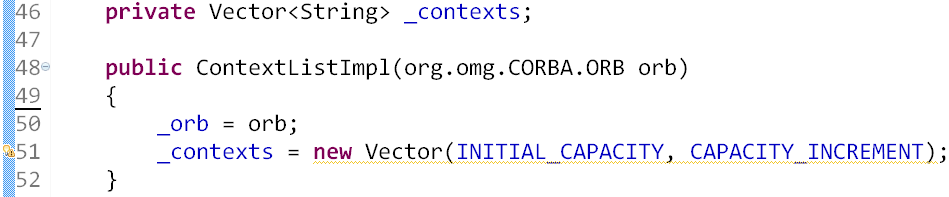
\includegraphics[width=3in]{figs/CMP2}
				\label{Comp2code}
			}}}
			\subfigcapskip = 1pt
			\subfigure[Text Description]{
				\fcolorbox{lightgray}{white}{\parbox{\dimexpr\linewidth-2\fboxsep-2\fboxrule}{
						
						{\scalebox{.8}{- Type safety: The expression of type Vector needs unchecked conversion}\\
							\scalebox{.8}{to conform to Vector<String>.} \\
							\scalebox{.8}{- Vector is a raw type. References to generic type Vector<E> }\\
							\scalebox{.8}{should be parameterized.}
						}
						
						\label{Comp2text}
					}} }
					
					\caption{A notification from the compiler about generics (CMP2).}
					\label{fig:CMP2} 
\end{figure}

For FindBugs, each task corresponded to a single notification.
All but one compiler task corresponded to a single notification; because the two notifications on CMP2 (Figure~\ref{fig:CMP2}) contribute to the same problem on the same line, we presented them as one task. 
Each EclEmma task consisted of coverage notifications for an entire class. 

\vspace{0.5em}
\noindent\textit{Data Collection \& Analysis.}
I transcribed each session and included descriptions of actions that a participant performed relevant to interpreting the notification. 
For example, if a participant navigated to different parts of the code but did not explicitly describe it, I added a description of that navigation to the transcript.


I analyzed each transcript using selective coding~\cite{corbin2014basics} to discover the challenges participants encountered with the goal of explaining the challenges programmers encounter. 
To identify a challenge, observing tool use as communication, I used Mustajoki's proposed model of (mis)communication to determine when a miscommunication-related challenge occurred~\cite{mustajoki2008modelling}. 
I created three criteria for identifying a challenge: 1) the participant explicitly states a challenge, 2) is unable to explain the notification, or 3) has to take steps, outside of reading the notification, to deduce the problem.

The coding process was completed by two researchers, myself and a co-author on the submitted work, and in two phases. In phase 1, we each coded all the transcripts individually using the criteria above. In phase 2, we reconvened to merge our codes and check for disagreements. Of the 404 codes we originally extracted, we disagreed on 82 (20\%). 
To resolve our disagreements, we referred to our criteria; if we could not come to an agreement regarding the code fitting the criteria, we removed the statement from our data set. For four sessions, we had no disagreement.
In the end, we identified 322 codes. I put each code onto a note card, along with the participant and tool being used. 

Using the note cards created during the coding process, I completed a card sort using a methodology similar to that of Mu\c{s}lu and colleagues~\cite{Muslu:2014:Transition}. 
The goal of this card sort was to identify themes based on our codes. 
I completed the card sort with four other researchers (also co-authors on the submitted work) and in three phases.
In phase 1, we sorted all cards into high-level themes; each card could only go in one theme. 
Phase 2 focused on determining where high-level themes could be broken down into lower-level themes.
In phase 3, we focused on making sure that each card was in the best fitting theme. During this phase, we also clarified theme definitions and made note of example statements to represent each theme.

%Because one my criteria is participant inability to explain a notification, any actions or statements made surrounding that occurrence was included in the card sort. Upon reflection, some emergent themes took the form of consequences of being unable to explain rather than challenges that led to inability to explain, such as notification resolution without understanding and lack of trust in the tool, therefore I will not discuss them in relation to this study. I likewise do not discuss the emergent theme of tool feature requests.

\def\toggle{
	\begin{scope}[ocg={name=test1, ref=t1, status=visible}]
		\node[inner sep=0pt] (svgPDF) at (0,0)
		{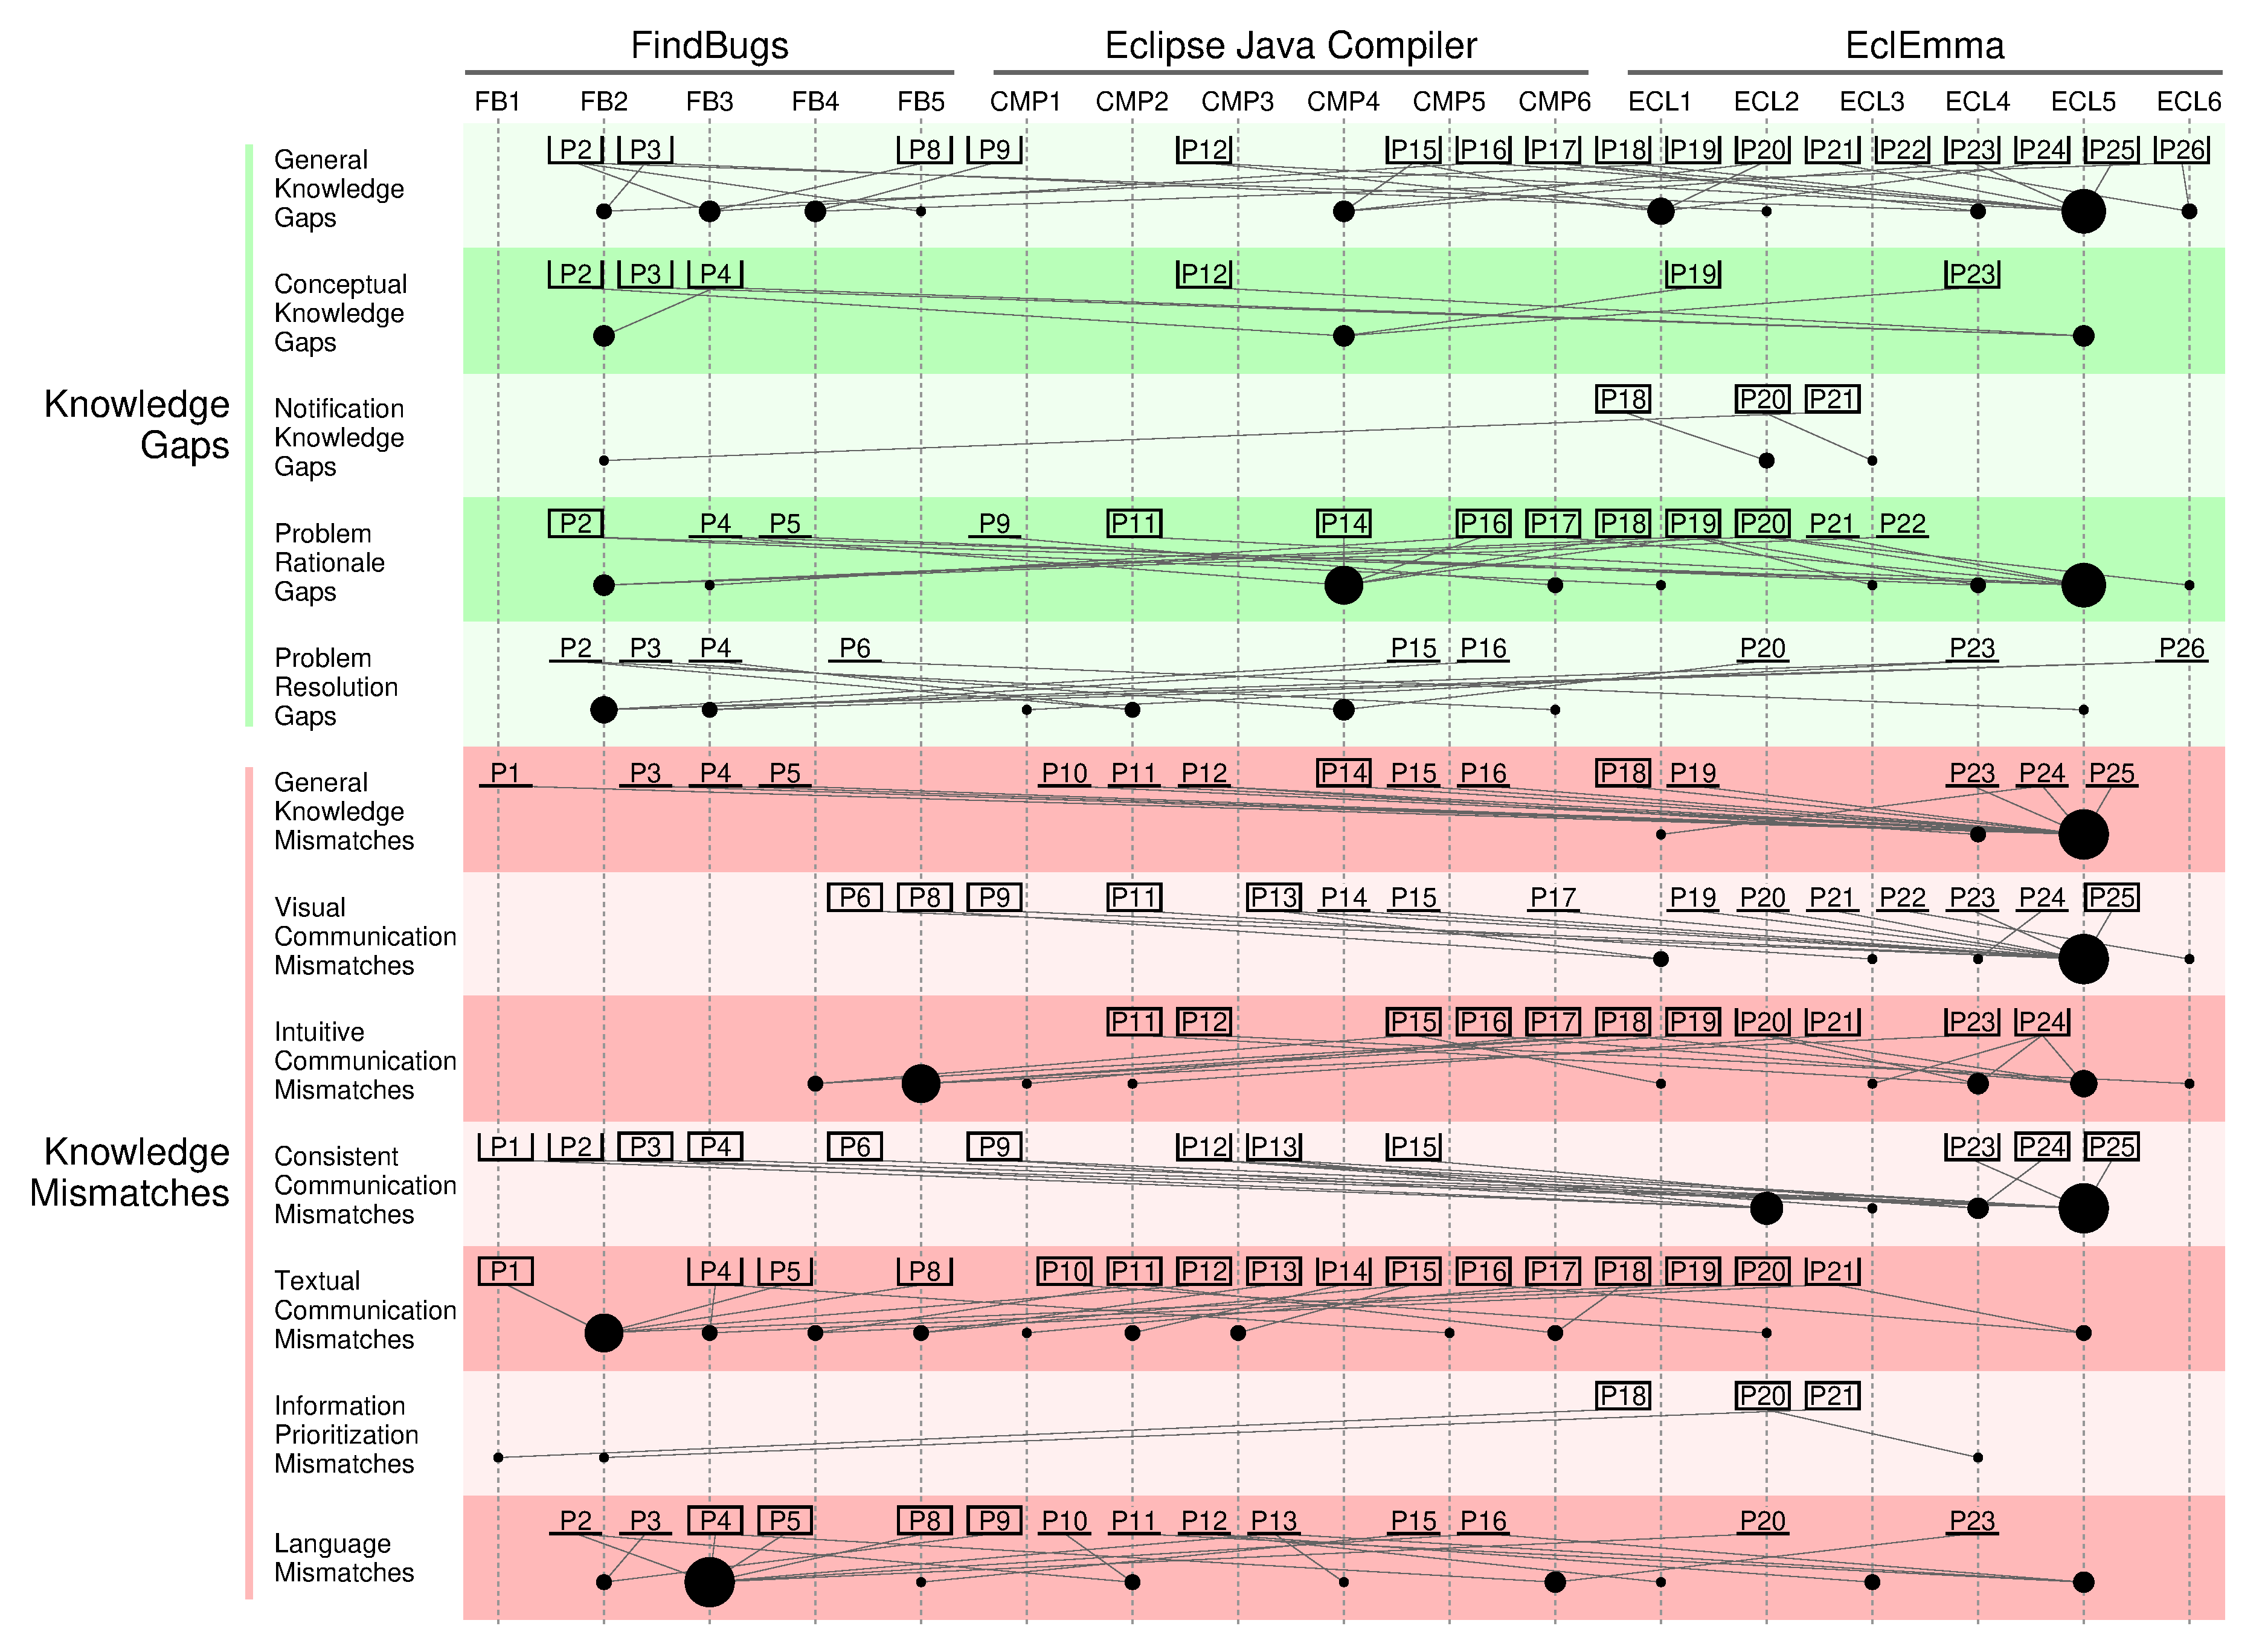
\includegraphics[width=\textwidth]{figs/Issues_Full_12.pdf}};
	\end{scope}
	\begin{scope}[ocg={name=test2, ref=t2, status=invisible}]
		\node[inner sep=0pt] (svgPDF) at (0,0)
		{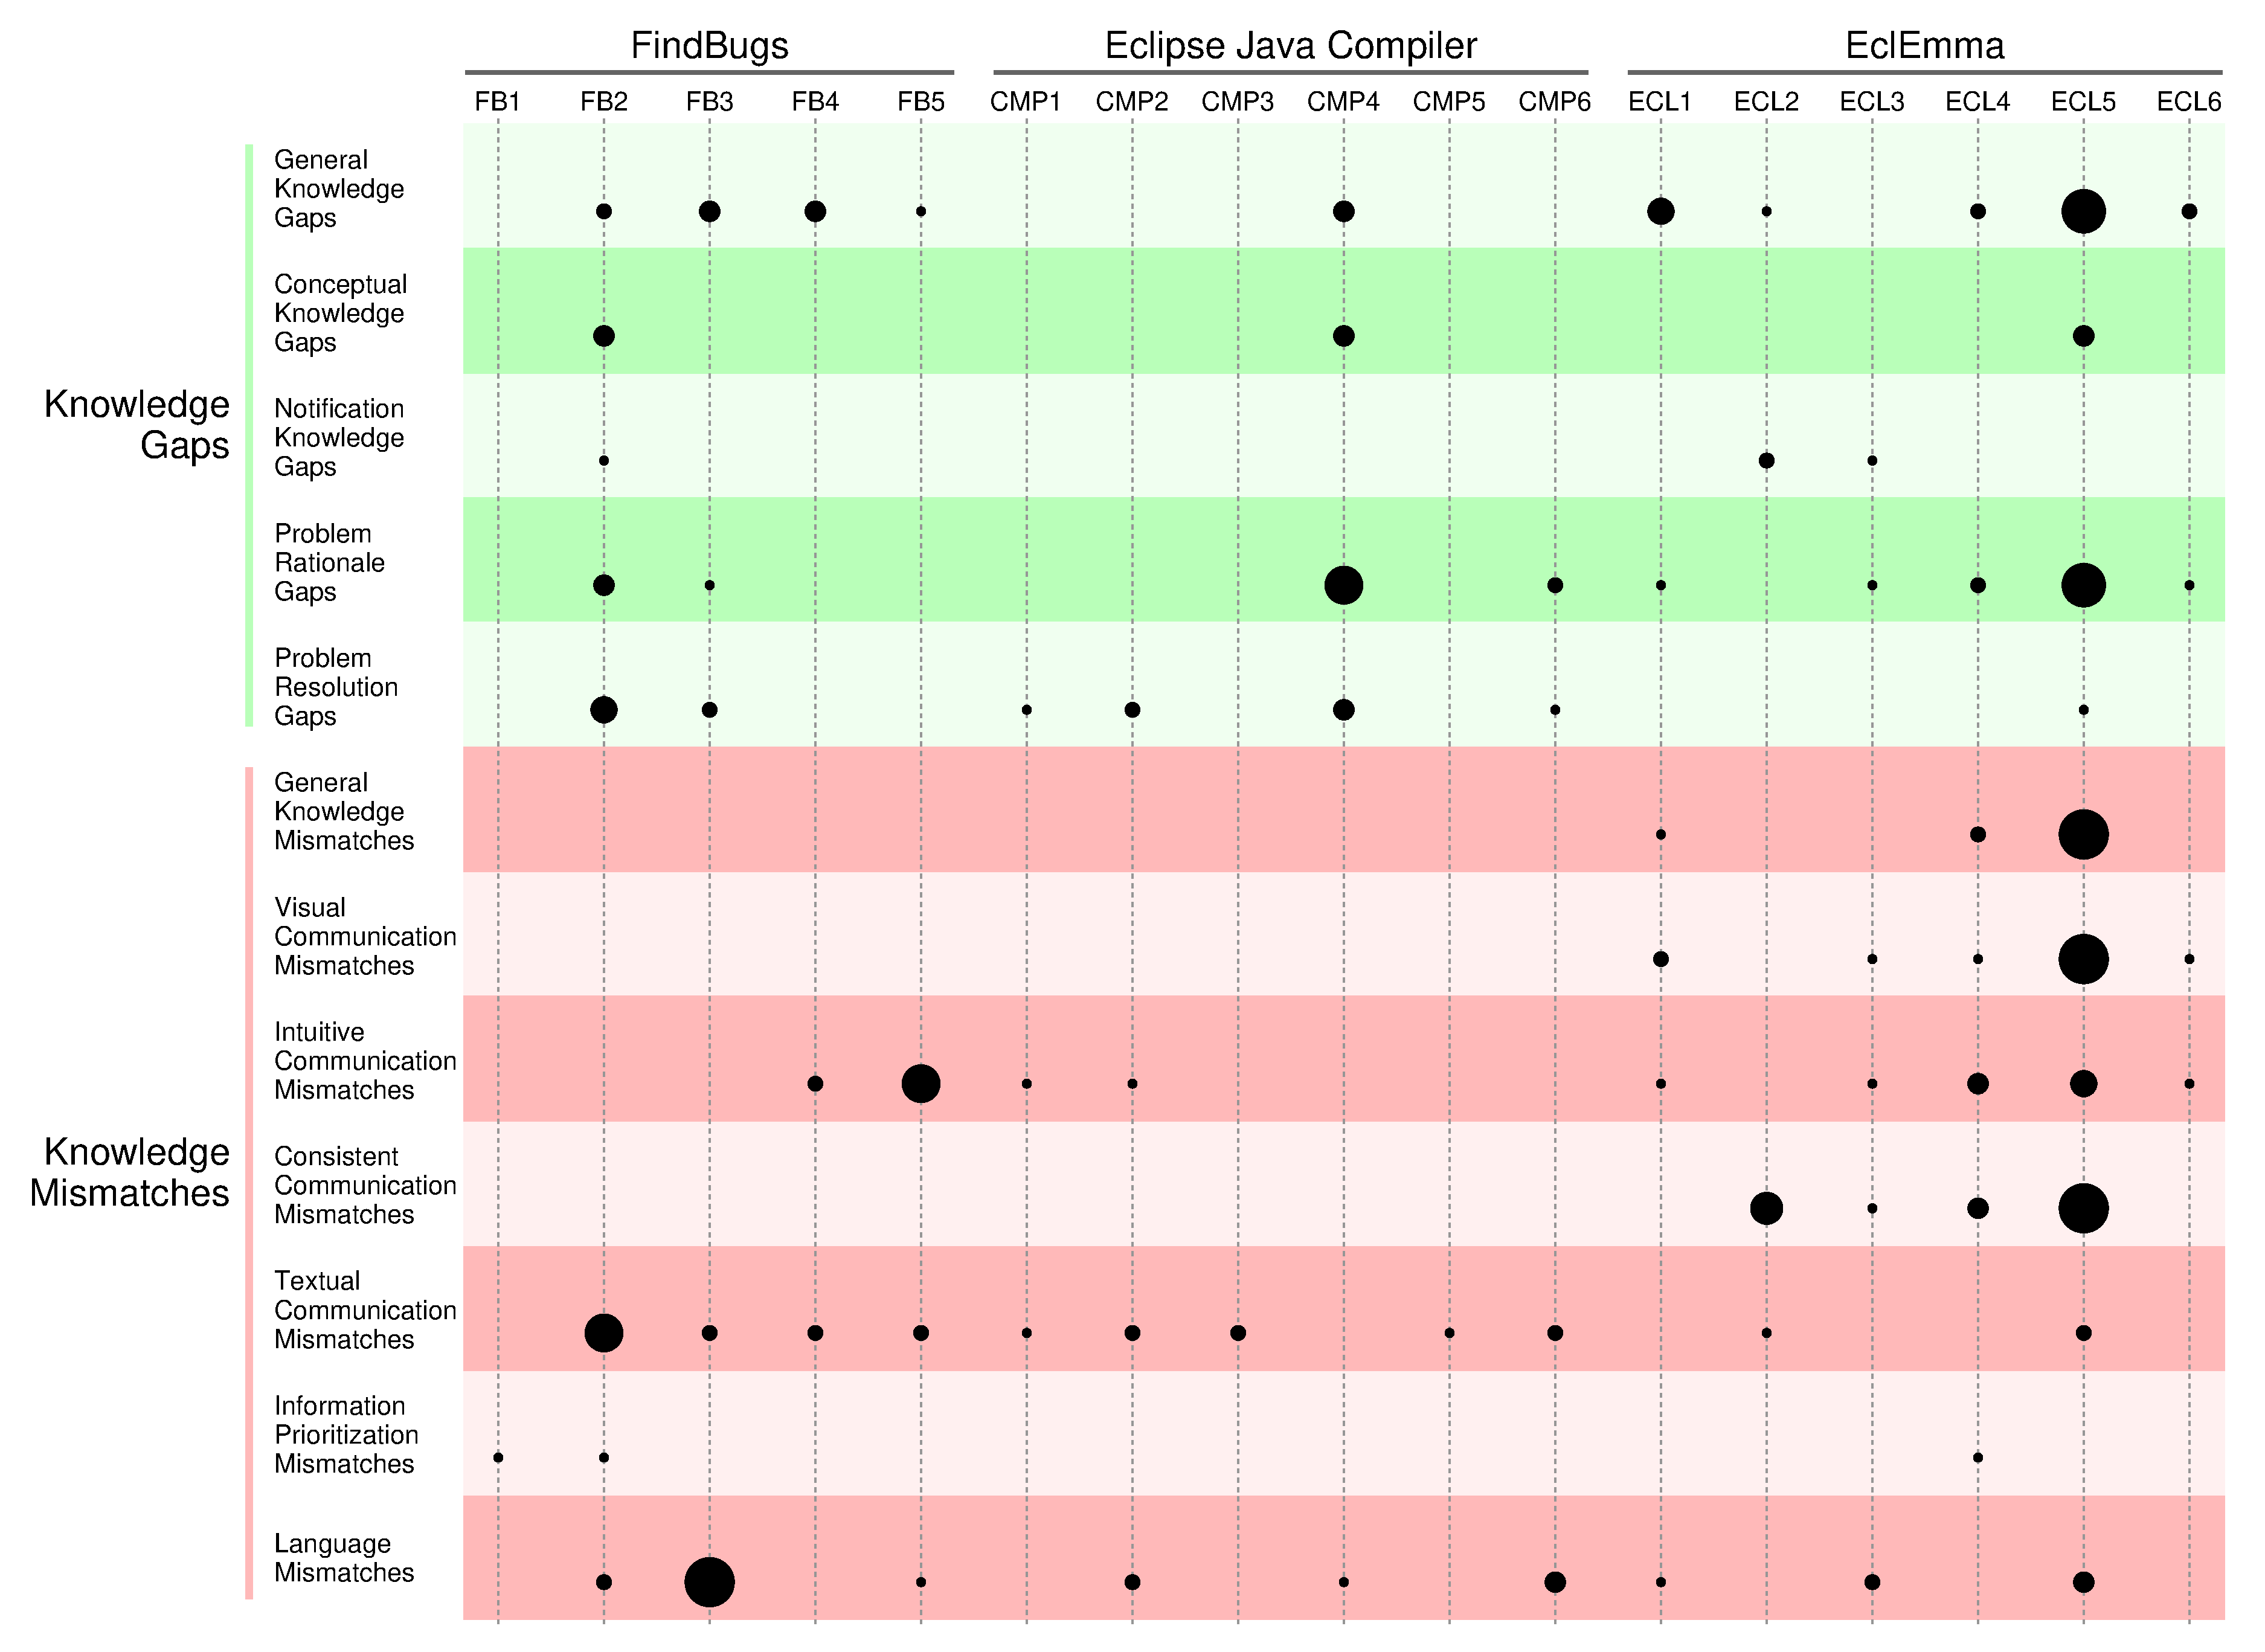
\includegraphics[width=\textwidth]{figs/Issues_Challenges_12.pdf}};
	\end{scope}
	\node[draw,switch ocg={t1 t2}] at (0,-5) {Hide/Display Details};
}

\begin{figure*}[ht]
	\centering
	\begin{tikzpicture}
	\toggle
	\end{tikzpicture}
	\caption{Distribution of challenges encountered and notifications that caused them.}
	\label{fig:results}
\end{figure*}

\subsubsection{Participants.} I conducted this study with 26 undergraduate students (10), graduate students (6), and professional developers(10), with varying amounts of development and tool usage experience. Three graduate students reported having industry experience. I recruited participants using mailing lists, classroom recruitment, and personal contacts.
Ten participants had prior experience using EclEmma. Nineteen participants had prior experience with FindBugs. All participants had experience with the Eclipse Java compiler.

\subsubsection{Results.} 
Based on findings from the study, I propose the following theory:

\begin{quotation}
	\noindent
	\emph{The challenges developers encounter when interpreting program analysis tool notifications are caused by gaps and mismatches between developer knowledge and how notifications communicate information.}
\end{quotation}

The kinds of challenges developer encountered during this study are shown in  Figure~\ref{fig:results}.\footnote{Credit for the creation of this figure goes to Sarah Elder, a co-author on this work.}
Vertical lines represent the tasks and the horizontal bars indicate challenges.
The different size dots indicate how many participants encountered challenges with that notification in that theme. 
The smallest dot represents one developer and the largest dot represents eight or more developers.
Diagonal lines map participants to the challenges interpreting that notification.
\setlength\fboxsep{1pt}
When opened in Adobe Acrobat, clicking \framebox{``Hide/Display Details''} in Figure~\ref{fig:results} interactively toggles between showing and hiding this mapping. 

Green challenges are caused by \emph{knowledge gaps} in what the developer knows and red challenges are caused by \emph{knowledge mismatches} between what the developer knows and how the tool communicates about those concepts.
These findings align with prior research that suggests one barrier for end-user programmers when using programming environments is ability to understand the code and errors associated with the code~\cite{ko2004six}. My research builds on these findings by identifying what causes inability to understand the notifications that appear in developers' source code.  


% model building (completed)
\subsection{Can we use developer experience to predict knowledge? [Predictions]\protect\footnote{Publication: Johnson, B., Pandita, R., Murphy-Hill, E., Heckman, S., Menzies, T., Predicting Developer Conceptual Knowledge Using Public Git Repositories. VL/HCC 2016 (in submission)}}\label{subsec:s3}

\subsubsection{Study rationale.}
The challenges developers encounter when interpreting tool notifications stem from the one-size-fits-all nature of tool notifications, despite the differences in what developers know and do not know.
Communication between notifications and developers can be improved if the notifications could adapt to the developer based on the developer's knowledge of programming concepts.
This proposition is based on constructivism, a verbal communication theory that suggests awareness of how the audience might react to a message improves communication~\cite{griffin2011first}. For this to be possible in the context of tool use, tools need a way of knowing what concepts the developer knows and do not know.
I implemented and evaluated an approach that uses concept inventories, a method used in education research for assessing conceptual knowledge~\cite{tew2010assessing}, and explores the possibility of providing knowledge information to tools in the form of concept knowledge models. 
The goal of this study was to develop and assess an approach for developing models that predict knowledge of programming concepts that appear in tool notifications based on concept-specific code the developer has written. 
%We designed a concept inventory to assess conceptual knowledge and collected source code relevant to the Java concept of generics from 24 developers. We used unsupervised learning to determine a model that accurately predicts developer knowledge.
%The main contributions of this paper are: 1) an approach for assessing developer conceptual knowledge using concept inventories and 2) an approach for modeling developer conceptual knowledge based on concept-specific code written by a given developer.

\subsubsection{Hypotheses.}

\begin{labeling}{hypotheses}
	\item [H\textsubscript{1}] We can predict conceptual knowledge using source code as a primary source of developer data.
	\item [H\textsubscript{2}] Concept-specific code increases model accuracy and precision compared to a model that uses lines of code (LOC) only.
\end{labeling}

\subsubsection{Approach.}
% TODO add mention of pilot??
Below I outline the approach I developed; research materials are available on-line.\footnote{http://www4.ncsu.edu/~bijohnso/apatian.html}

\vspace{0.5em}
\noindent\textit{Assessing \& Encapsulating Conceptual Knowledge.}
To assess \& encapsulate developer knowledge as the dependent variable for the models, I borrowed from computer science education literature and developed a concept inventory~\cite{tew2010assessing}. 
To determine the questions for the inventory, I identified key generics concepts using the Oracle Java Tutorial on Generics\footnote{\url{http://docs.oracle.com/javase/tutorial/java/generics/}} to find and map the relationships between generics concepts and ancestor concepts; if Lesson 5 built on top of Lesson 1, I considered Lesson 5 an ancestor of Lesson 1. For example, based on the generics tutorial, I labeled Upper Bounded Wildcards as an ancestor concept to Wildcards. To ensure I covered all concepts, I checked other Java generics tutorials; no new concepts emerged from this process.

Once I had the key concepts, I came up with at least 1 question for each level of revised Bloom's taxonomy, based on my test specification, using examples found in work by Nelson~\cite{nelson1967testing} and Thompson and colleagues~\cite{thompson2008bloom}.
From this process, I derived 11 questions.
I piloted my initial set of questions with 11 developers and students at NC State University. 

Next, to test the validity and reliability of the concept inventory, I used item and distractor analysis in R. Item analysis determined if the items on the inventory are valid methods of assessment; from this process I eliminated 1 question, which yielded a final set of 10 questions.  Distractor analysis determined if the options provided for a given question are fair and if the incorrect options contribute to the quality of the inventory; because each option was selected at least once for each inventory item, and most often the correct option was chosen, I kept all response options for each inventory item.
I did another pilot once I established validity and reliability.

I also asked participants to self-report how much they know about generics to assess the possibility to use self-report as a proxy for knowledge and experience. However, developers almost always over- or underestimated their knowledge based on my assessment, matching concept inventory scores 18\% of the time. This aligns with existing research that suggests objective knowledge, based on a factual test, may be better for task performance oriented measures, such as ability to understand concepts~\cite{cole1992exploring,raju1995differential}. Based on these findings, and existing research, I used concept inventory scores rather and collect source code as a proxy for experiences that led to knowledge~\cite{argote2011organizational,raju1995differential} rather than self-report scores alone.

\vspace{0.5em}
\noindent\textit{Source Code Analysis.}
To test my hypotheses, I chose Java generics as the initial concept. I made this decision primarily because generics requires motivation on behalf of the developer to explore beyond the basics and is a concept appears in notifications across program analysis tools. When we say motivation, we refer to an intrinsic motivation to learn that stems from an interest in learning~\cite{krapp1999interest,hall2008we}.		
Another advantage to using a concept like generics to test my hypotheses is that it is multi-faceted; there are enough features of and ways to use generics for there to be relationships that I can explore and use to generalize for applicability to other concepts.~\footnote{Although this approach is evaluated on what I would consider a complex concept, this approach will also work for simpler concepts where, based on the language features, there may be fewer options for advanced learning about the concept.}

To determine the independent variables for my model, I analyzed for code contributions and assigned them to developers using version control. 
I built a Java source code analyzer that analyzes code bases for concept-specific code using the Eclipse JDT ASTParser. 
One example of generics-specific code is a generic type declaration ((\texttt{public class <T> Box})).
I used code bases in repositories to determine what developer made what contribution via the commit history. 
I chose the versioning platform Git\footnote{\url{https://git-scm.com/}} so I could use JGit,\footnote{\url{http://eclipse.org/jgit/}} which allows for manipulation of Git repositories via Java code, along with ASTParser to analyze for developer code contributions.

To test H\textsubscript{1} and H\textsubscript{2}, I collected concept-specific code and manually collected LOC added from GitHub, a social coding site where developers can create and maintain Git repositories.\footnote{\url{http://www.github.com}} To determine LOC, I manually checked the contributions reported by GitHub for each developer's repositories. To determine what concept-specific code to analyze for, I used the same key concepts identified for the concept inventory (i.e. generic type declarations). I collected 11 different types of generics usage, such as generic type declarations and usage of the Wildcard (\texttt{?}) generic type.\footnote{The repository that holds the analyzer can be found at \url{https://github.com/brittjay0104/APATIANproto.git}.}

I also used version control to detect when the most recent contribution of each type of generics usage was made; prior analyses indicated time may play a factor in how predictive code contributions are~\cite{johnson2015bespoke}.
The output of my analyzer for each repository is an occurrence count for all contributed generics code and when the most recent contribution for each type of generics was.
To determine which types of generics usage might be more advanced than others, I used the output from analyses to create a hierarchy of generics feature usage. The feature hierarchy, along with a description of the creation process and usage, can be found on-line.\footnote{http://www4.ncsu.edu/~bijohnso/docs/feature-map.pdf}

% FEATURES AND HEURISTICS
To increase the generalizability of the model to other concepts, I characterized the independent variables for the model by grouping the types of generics collected based on \emph{features} of the data. For example, a feature of type declarations and type parameter methods (\texttt{public <T> method()}) that groups them together is that the developer wrote new generic code for use by other developers, rather than using existing generic code.
The set of features I identified among the data are as follows:
\begin{itemize}
	\item \textbf{Declared Generics:} I computed Declared Generics by adding together counts from the types of generics where the developer wrote new generic code for use by themselves or others (i.e. type declarations).
	\item \textbf{Used Generics}: I computed Used Generics by adding together counts from the types of generics that are ways to use generics, as opposed to contributing to a new generic type (i.e. method invocations).
	\item \textbf{Levels of Generics Usage:} I computed the Levels of Generics Usage by adding together counts from the types of generics that would be considered on a basic, intermediate, or advanced level of usage. I used the feature hierarchy discussed above. 
\end{itemize}

\noindent I also defined two \emph{heuristics} to apply to the feature groups:

\begin{itemize}
	\item \textbf{Recency:} The recency heuristic takes each of the features and multiplies each value by 1.0 if the most recent contribution was made in the last week, 0.8 if between one week and one month, 0.6 for 1--6 months, 0.4 for one year, and 0.2 for more than one year.
	For example, if, the total number of declarations made by a developer (Declaration heuristic) is 198 and the most recent declaration was written between one week and one month, the Declaration Recency (DeclRecency) heuristic value would be 158.4 (\(198 \times 0.8)\). 
	\item \textbf{Natural Log:} This heuristic calculates natural log of each feature group before and after the recency heuristic is applied.
\end{itemize}
%	we were able to build models with useful levels of precision and recall
	
I applied natural log to the data following the reasoning of Fritz and colleagues, who used natural log in their models to account for the potential for large differences in variable values~\cite{fritz2010degree}. For example, some repositories returned counts in the thousands for class instantiations but counts of zero for explicit method invocations; this might cause our model to put more weight on the contribution of feature groups and heuristics that include class instantiations than it truly contributes.
I used both the \emph{features} and \emph{heuristics} defined above to determine the independent variables for analyses.

\vspace{0.5em}
\noindent\textit{Data Analysis.}
To define the relationship between the dependent and independent variables, I used Weka~\cite{Hall:2009:WDM:1656274.1656278} for access to machine learning algorithms suitable for my small dataset of 24 GitHub developers; only 24 developers completed the concept inventory, which was necessary for developing and evaluating my current approach. 
Specifically, I used Weka's J48 classifier~\cite{witten1999weka} to create decision trees.

To select the independent variables best suited for the model, I used Correlation-based Feature Selection (CFS) in Weka. This analysis runs k-fold cross validation using the independent variables passed in; to lower the potential for a model with overestimation bias, I maintained even and sizable chunks by using 4-fold cross validation.
CFS evaluates each attribute on its predictive ability and uses cross-validation to indicate how stable the best subset of variables is based on how many folds the variable appeared in.
For increased model stability, I selected the variables that appeared in more than one fold.

\subsubsection{Results.}

\begin{table}[h]
	\centering
	\caption{Precision, Recall, and F-Score for Beginner Classification}
	\label{tab:beginner}
	\begin{tabular}{llll}
		\hline
		\multirow{2}{*}{}                                                    & \multicolumn{3}{c}{\textbf{Beginner}}                   \\ \cline{2-4} 
		& \textit{Precision} & \textit{Recall} & \textit{F-Score} \\ \hline
		\textbf{LOC}                                                         & 0.5                & 0.333           & 0.4              \\
		\textbf{DeclRecency}                                                 & 0.667              & 0.333           & 0.444            \\
		\textbf{\begin{tabular}[c]{@{}l@{}}DeclRecency +\\ LOC\end{tabular}} & 0.625              & 0.833           & 0.714       \\
		\hline    
	\end{tabular}
\end{table}

\begin{table}[h]
	\centering
	\caption{Precision, Recall, and F-Score for Intermediate Classification}
	\label{tab:intermediate}
	\begin{tabular}{llll}
		\hline
		\multirow{2}{*}{}                                                    & \multicolumn{3}{c}{\textbf{Intermediate}}               \\ \cline{2-4} 
		& \textit{Precision} & \textit{Recall} & \textit{F-Score} \\ \hline
		\textbf{LOC}                                                         & 0.636              & 0.778           & 0.7              \\
		\textbf{DeclRecency}                                                 & 0.727              & 0.889           & 0.8              \\
		\textbf{\begin{tabular}[c]{@{}l@{}}DeclRecency +\\ LOC\end{tabular}} & 0.75               & 0.667           & 0.706        \\   
		\hline
	\end{tabular}
\end{table}


\begin{table}[h]
	\centering
	\caption{Precision, Recall, and F-Score for Advanced Classification}
	\label{tab:advanced}
	\begin{tabular}{llll}
		\hline
		\multirow{2}{*}{}                                                    & \multicolumn{3}{c}{\textbf{Advanced}}                   \\ \cline{2-4} 
		& \textit{Precision} & \textit{Recall} & \textit{F-Score} \\ \hline
		\textbf{LOC}                                                         & 0.875              & 0.875           & 0.875            \\
		\textbf{DeclRecency}                                                 & 0.778              & 0.875           & 0.824            \\
		\textbf{\begin{tabular}[c]{@{}l@{}}DeclRecency +\\ LOC\end{tabular}} & 1                  & 0.875           & 0.933     \\
		\hline      
	\end{tabular}
\end{table}


\begin{table}[h]
	\centering
	\caption{Total Precision, Recall, and F-Score}
	\label{tab:total}
	\begin{tabular}{llll}
		\hline
		\multirow{2}{*}{}                                                    & \multicolumn{3}{c}{\textbf{Total}}                      \\ \cline{2-4} 
		& \textit{Precision} & \textit{Recall} & \textit{F-Score} \\ \hline
		\textbf{LOC}                                                         & 0.684              & 0.696           & 0.683            \\
		\textbf{DeclRecency}                                                 & 0.729              & 0.739           & 0.715            \\
		\textbf{\begin{tabular}[c]{@{}l@{}}DeclRecency +\\ LOC\end{tabular}} & 0.804              & 0.783           & 0.787      \\
		\hline     
	\end{tabular}
\end{table}


Based on developer classifications and the set of independent variables, CFS identified two variables that fit my variable selection criteria: LOC and DeclRecency.  	
I created three decision tree models: 1) LOC only (Figure~\ref{fig:LOC}, 2) DeclRecency only (Figure~\ref{fig:decl}, and 3) LOC \(+\) DeclRecency (Figure~\ref{fig:declLOC}. I created a model based on LOC only to test H\textsubscript{2}. 
To further explore how each affects overall model accuracy and precision for H\textsubscript{1} and H\textsubscript{2}, I created a model using both LOC and DeclRecency.
The values for each model's \emph{precision}, \emph{recall}, and \emph{F-Score} values are shown in Table~\ref{tab:beginner} (Beginner), Table~\ref{tab:intermediate} (Intermediate), Table~\ref{tab:advanced} (Advanced), and Table~\ref{tab:total} (Total).
%	We observed the model's ~\cite{olson2008advanced}; 

% H1 --> can use source code
\vspace{0.5em}

\begin{figure} [h]
	\centering
	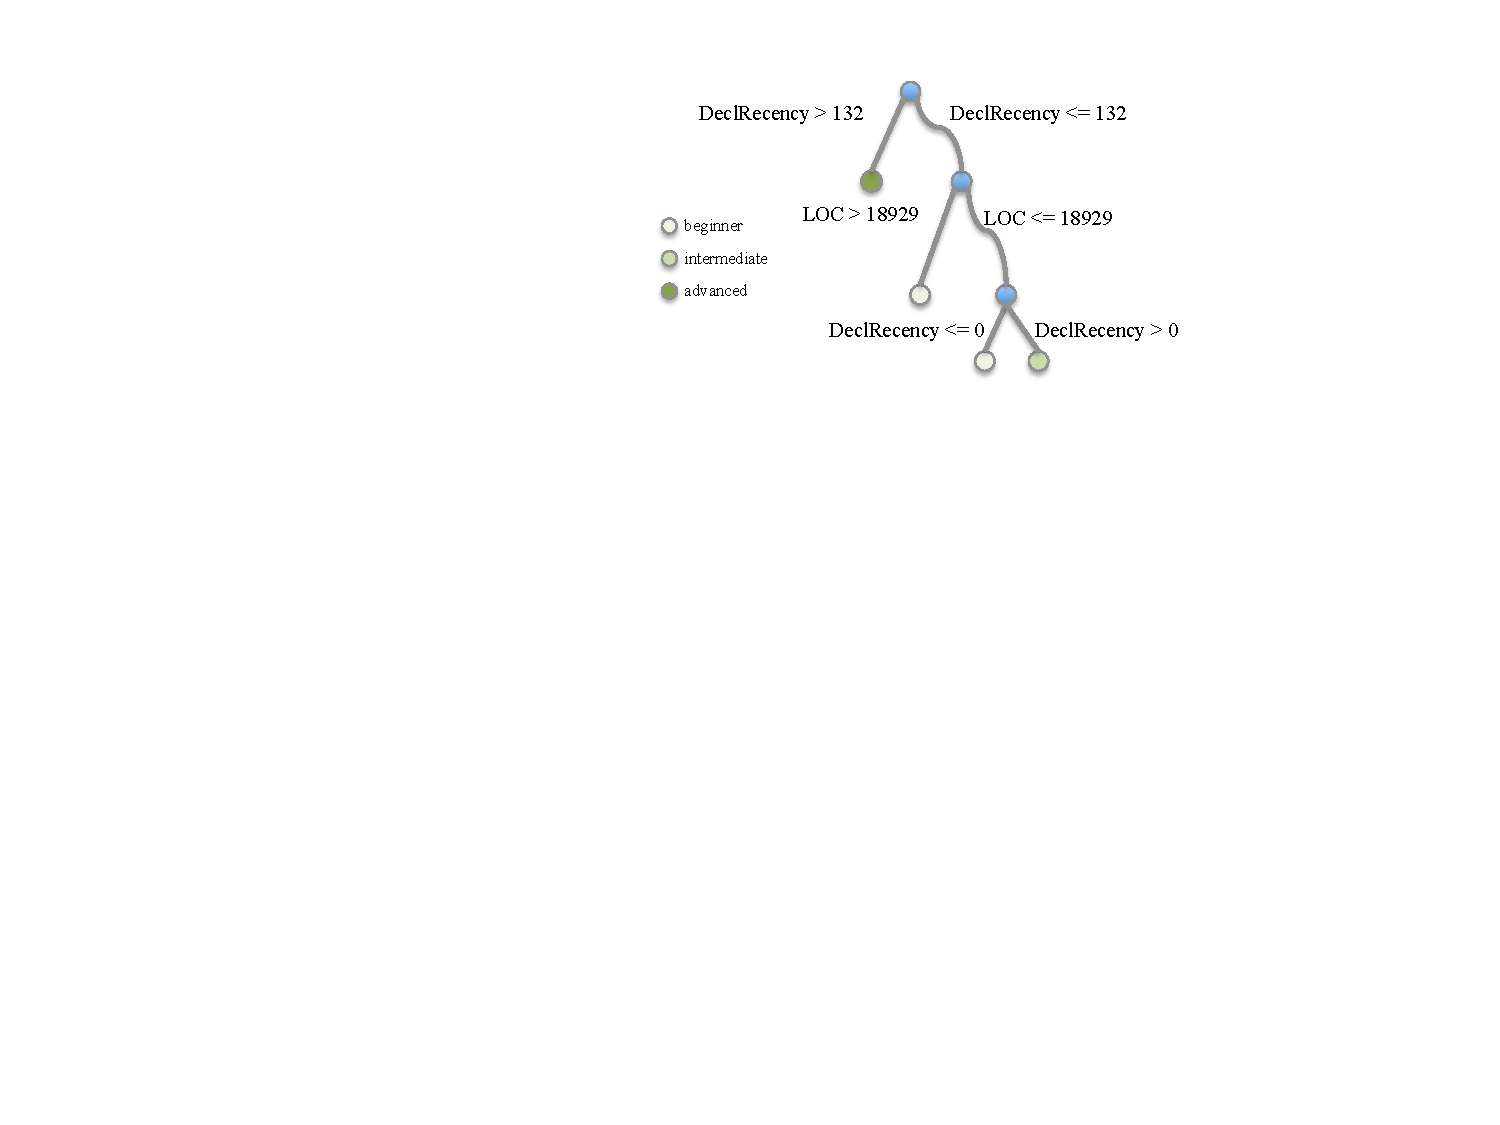
\includegraphics[width=4in]{figs/decl-LOC.pdf}
	\caption{Decision tree model using DeclRecency and LOC as independent variables.}
	\label{fig:declLOC}
\end{figure}

\begin{figure} [h]
	\centering
	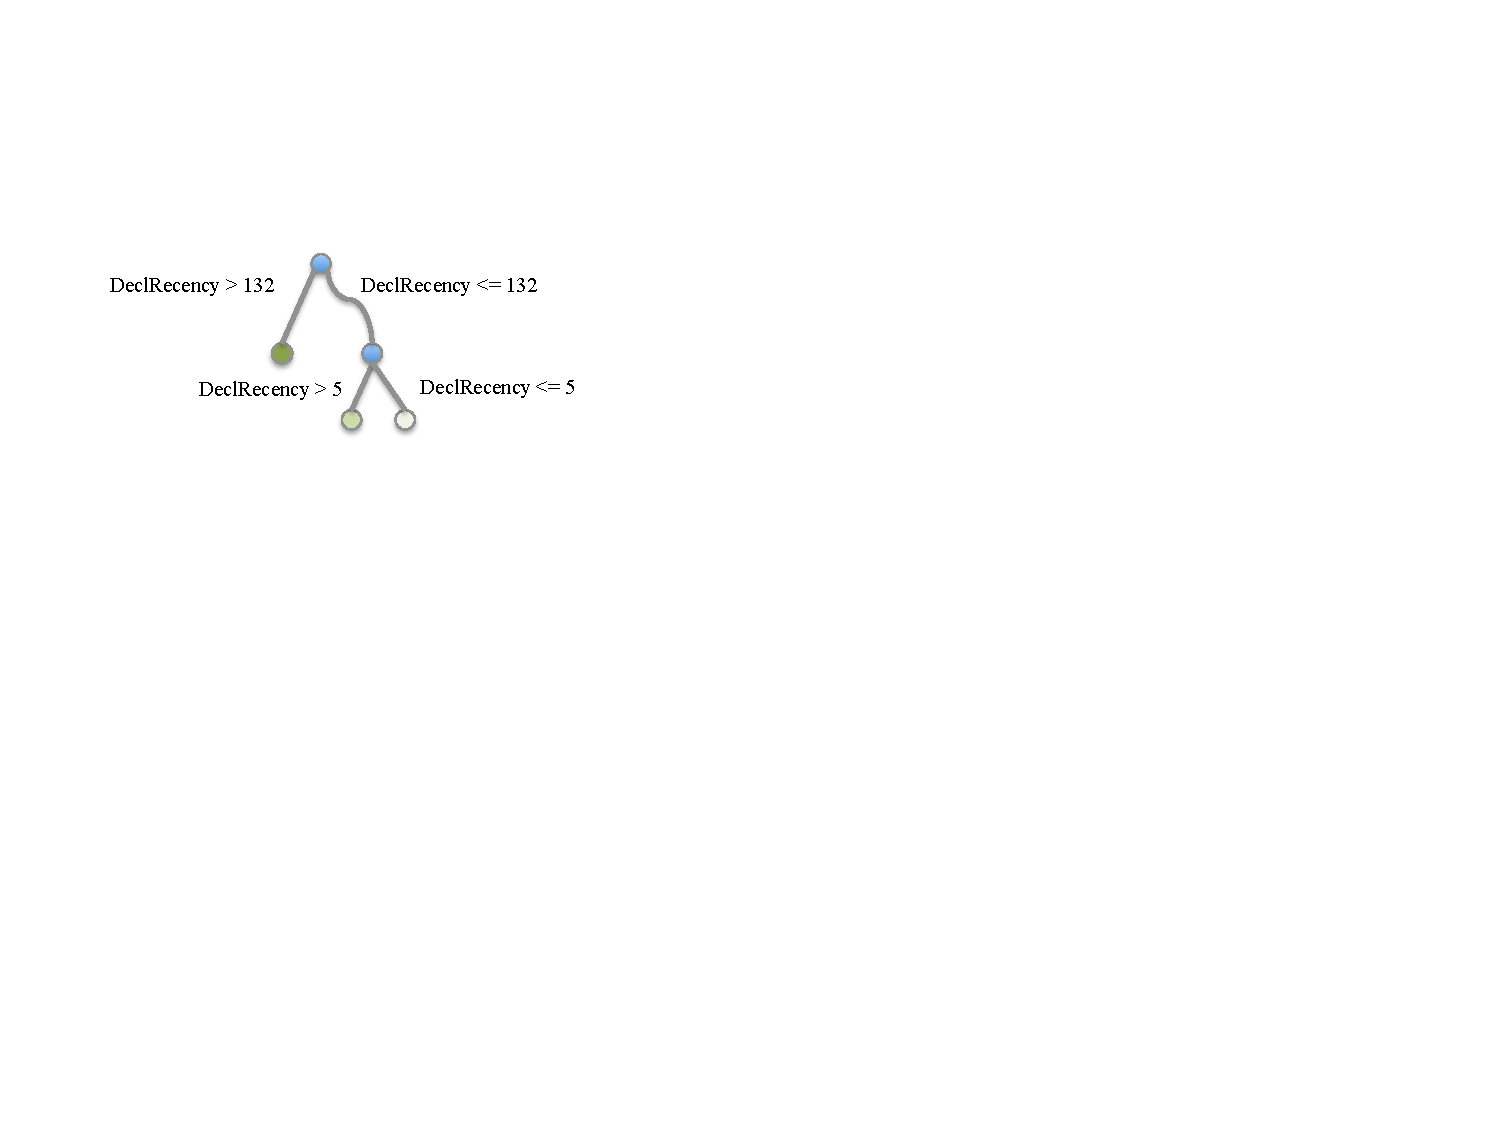
\includegraphics[width=3.5in]{figs/decl.pdf}
	\caption{Decision tree model using DeclRecency as the independent variable.}
	\label{fig:decl}
\end{figure}

\begin{figure} [h]
	\centering
	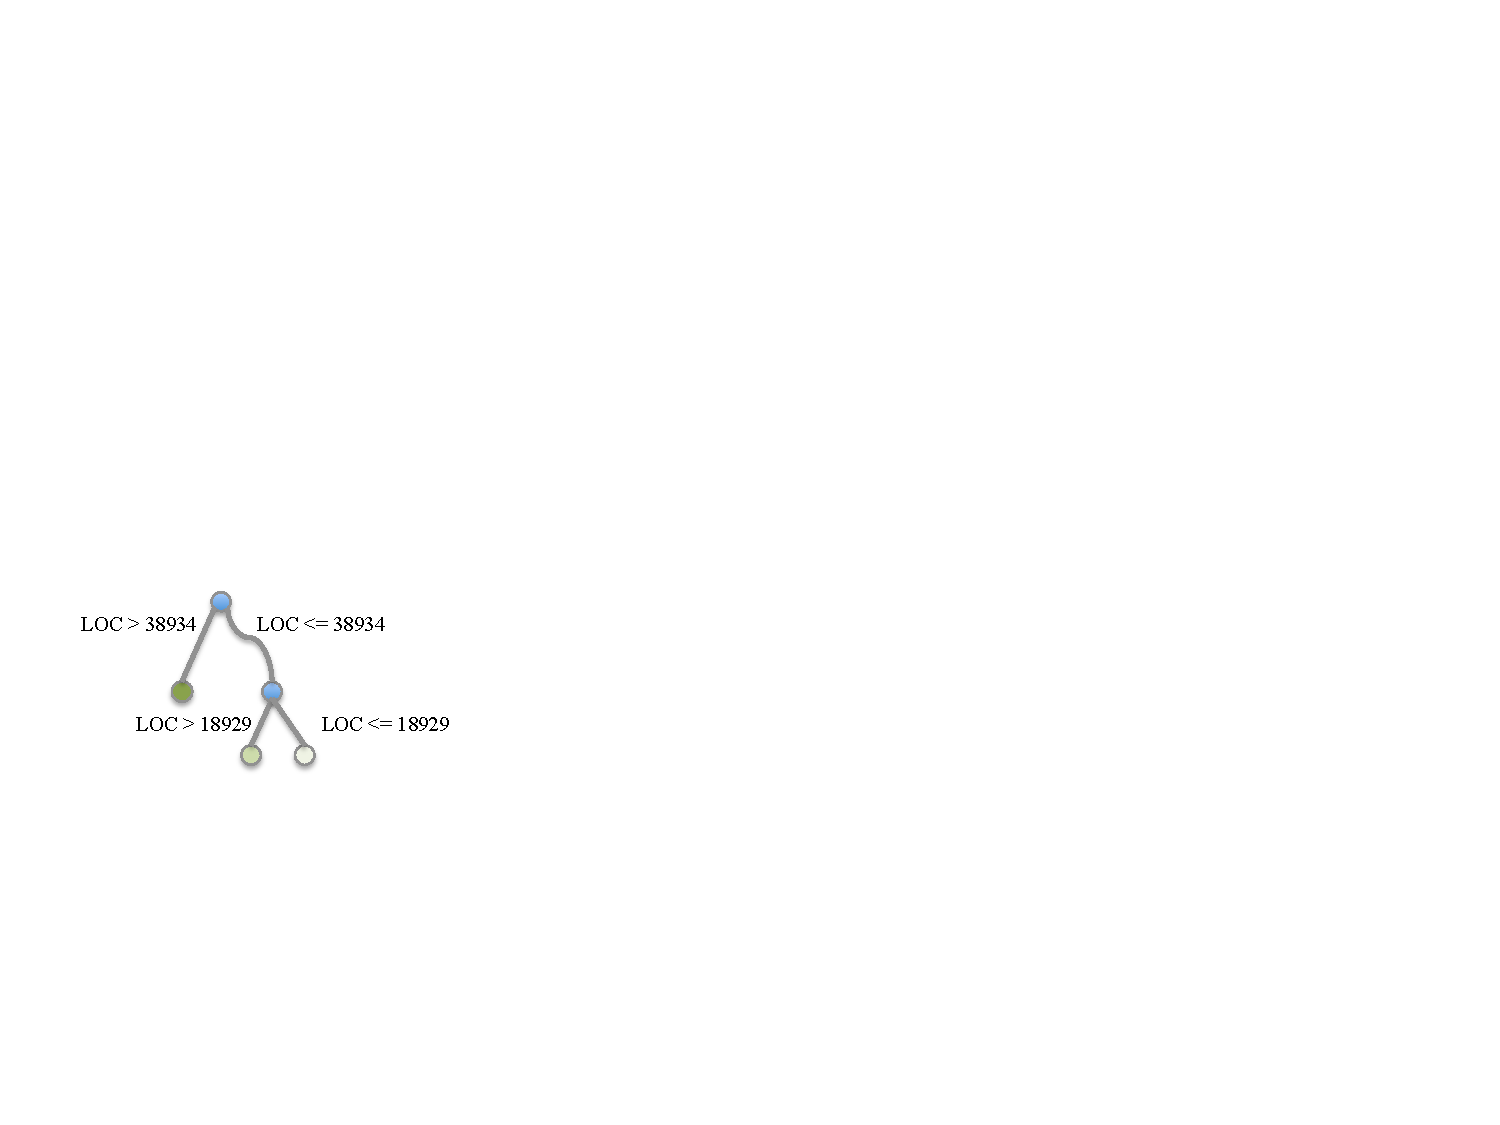
\includegraphics[width=3in]{figs/LOC.pdf}
	\caption{Decision tree model using LOC as the independent variable.}
	\label{fig:LOC}
\end{figure}

\noindent\textbf{My findings support H\textsubscript{1}: it is possible to predict conceptual knowledge using source code as a primary source of developer data.}\\
All three models correctly classified developers more often than not (LOC = 70\%; DeclRecency = 74\%; Combination = 78\%); in fact, by combining LOC with DeclRecency, the accuracy of classification increased by 4\%. This increase may be due to the fact that, as existing research suggests, all experiences contribute to overall knowledge~\cite{argote2011organizational,raju1995differential}. Similarly, general coding experience seems to also contribute to conceptual knowledge.

Based on the models shown in Figure~\ref{fig:declLOC} and Figure~\ref{fig:decl}, how recently code contributions are made also affect conceptual knowledge. Based on the recency heuristic, a higher DeclRecency value suggest more recent code contributions. This suggests that determining a developer's knowledge of concepts may require both concept-specific declarations and recent experience with concept-specific declarations. 


% H2 --> concept-specific code better
\vspace{0.5em}

\noindent\textbf{My findings support H\textsubscript{2}: concept-specific code improves model performance compared to a model that uses LOC only.}\\
The LOC model's precision, recall, and F-Score suggest it may be better at classifying developers with advanced generics knowledge than the DeclRecency model (Figure~\ref{tab:advanced}). However, overall model accuracy is higher in the DeclRecency model (74\%) than the LOC model (70\%) (Table~\ref{tab:total}. There was also a slight performance increase overall, with increased precision and F-Score for beginner (\(+ 0.167\), \(+ 0.04\)) and intermediate (\(+ 0.09\), \(+ 0.1\)) classification and increased total precision (\(+ 0.05\)), recall (\(+ 0.04\)), and F-Score (\(+ 0.03\)). Also, as shown in Figure~\ref{fig:declLOC}, LOC only becomes relevant when classifying beginner and intermediate developers. This may be because beginner and intermediate developers do not declare enough generics to make an informed decision without some reference to the general experience they have.
Regardless, these findings suggest that although both LOC and concept-specific code can both be used to predict conceptual knowledge, concept-specific code increases overall model accuracy and precision.


\subsection{Does my prototype concept knowledge model generalize? [Generalize]} \label{subsec:s4}

\subsubsection{Study rationale.} Two important aspects to consider when developing a quality tool or approach are \emph{performance} and \emph{scalability}~\cite{fox2011performance}. 
However, when evaluating models, rather assessing scalability, researchers should assess model performance and \textit{generalizability}~\cite{forster2000key}. 
My previous study, \textbf{Predictions}, found that it is possible to assess, model, and accurately predict developer knowledge regarding Java generics (performance), based on the predictions of a prototype model (M1). However, it is not obvious if M1 generalizes to other concepts and developers.
The end goal is an approach that can be applied to any concept and be used to make predictions for any Java developer (scalable) while still performing at a high level. Therefore, I designed a study where I will explore the generalizability of M1 to other programming concepts and different sets of developers. 

\subsubsection{Research questions.}

\begin{labeling}{questions}
	\item [RQ1] To what extent does M1 generalize to developers outside the set used to create the model?
	\item [RQ2] To what extent does M1, and the approach used to create M1, generalize to concepts outside the concept used to create the model?
	\item [RQ3] What other factors may contributor to developer knowledge of programming concepts?
\end{labeling}

\subsubsection{Proposed methodology.}
I plan to explore the generalizability of, and refine, the approach that led to M1 by combining qualitative feedback with generalizability assessments. One of my ongoing (implicit) model refinement efforts is finding more developers for building and assessing M1 and, if needed, creating and evaluating new models.

\vspace{0.5em}
\noindent\textit{Generalizability Assessments.}
I built and evaluated M1 using the same set of developers. I plan to assess the generalizability M1 on other developers (RQ1) by making predictions using M1 with a separate set of developers. Doing so will allow me to observe the ability for M1 to generalize to a wide range of developers. 
To assess the generalizability of M1 in regards to other concepts (RQ2), I plan to develop new concept inventories and analyze participant repositories for concept-specific code pertaining to others Java concepts.

I plan to conduct these generalizability assessments using three concepts: operators, variables, and exceptions.
I chose three concepts to balance feasibility of completion within a reasonable timeframe (1 - 1.5 years) and confidence in generalizability outside of one concept or set of notifications.
I chose operators, variables, and exceptions as the three concepts I will use for my generalizability assessments because 1) there are notifications across tools pertaining to these concepts, 2) FindBugs, the tool whose notifications I will use in future evaluations, has notifications pertaining to these concepts~\footnote{http://findbugs.sourceforge.net/bugDescriptions.html}, and 3) notifications pertaining to these concepts appear in production software~\cite{ayewah2007evaluating}.

\vspace{0.5em}

\noindent\textit{Qualitative Data Collection \& Analysis.}
Although there is value in quantitative findings, my research experience suggests that there is a richness in qualitative data that cannot be achieved with quantitative data and analyses.
I chose the variables for M1 based on qualitative and quantitative findings; therefore, another way I plan to assess generalizability, and find opportunities for approach refinement, is by conducting short, semi-structured interviews with developers (10--20) regarding factors that contribute to their programming concept expertise (RQ3). 

Each interview will last approximately 30 minutes and will be divided into two phases: 1) the relationship between the code they write and their expertise regarding the concept and 2) other factors that contribute to their knowledge of programming concepts.  

To determine what factors developers consider as contributors to their knowledge, I plan to 1) code each transcript and 2) perform content analysis in R~\cite{RSoftware} on interview transcripts. Content analysis assumes that content most frequently mentioned is the most important. For example, if in multiple interviews participants discuss on-line programming forums, such as Stack Overflow, one item that content analysis may identify as important in relation to the topic being discussed, is on-line forums. In order to perform content analysis, I need well defined categories, such as on-line forum usage; this is where the coding process comes into play. Using a methodology similar to the ones in my previous research, I will code each transcript for statements pertaining to their knowledge of concepts and experiences that contributed knowledge for them. 

To validate source code as a factor, and other factors that emerged during the interviews, I plan to administer a survey to another set of developers (50--100). To encourage participation, and thereby increase the likelihood I will get a large set of responses~\cite{smith2013improving}, I plan to ask only one question: \emph{Which of the following contribute to your knowledge of programming concepts?}. I will include a definition and example of a programming concept so that participants are able to accurately respond. I will also communicate to their interests as developers, such as improvement of the tools available for the to use.
I will include each factor identified during the interviews as response options.
I will determine the factors that contribute most to developer knowledge by running various analyses using R with data from the survey. Findings from both the qualitative and quantitative analyses will serve to potentially confirm current model building efforts and inform future data analysis and model building efforts.

\subsubsection{Participants.} To increase the ability to compare M1 to future models, I plan to conduct this study with at least 25 GitHub developers. I plan to recruit participants by re-contacting participants from \textbf{Predictions}. As a back-up, I also plan to use mailing lists, personal contacts, and GitHub search to find developers. Because I already have a participant pool to re-sample, and a handful of participants that have expressed interest in continuing participation and helping with recruitment, I expect it will be faster and easier to acquire my goal of at least 25 participants.

\subsection{Are adaptive, knowledge-based notifications more effective than one-size-fits-all notifications? [SmartBugs]} \label{subsec:s5}
\subsubsection{Study rationale.}
Based on findings from previous studies, I proposed that communication between tools and developers can be improved if rather than using one-size-fits-all notifications, tools used knowledge-based notifications~\cite{johnson2015bespoke}. Knowledge-based notifications would use concept knowledge models. We found that communication theory applies directly to tool use, therefore constructivism communication theory should also apply~\cite{griffin2011first}. 
I have explicitly assessed the applicability of general communication theory to tool use (Section~\ref{subsec:s2}), however, I have not explicitly assessed the applicability of constructivism to notification and tool design. Therefore, the goal of this study is to assess whether knowledge-based communication, in regards to tool use, is better than one-size-fits-all communication.

\subsubsection{Research questions \& Hypothesis.}

\begin{labeling}{questions}
	\item [RQ1] How does existing notification design, problem solving, and debugging research map to differences in developer knowledge?
	\item [RQ2] Are there differences in notification design expectations across developers with differing knowledge?
	\item [H\textsubscript{1}] Adaptive, knowledge-based notifications require less time and context-switching for notification understanding and resolution than one-size-fits-all notifications.
\end{labeling}

\subsubsection{Proposed methodology.}
To answer RQ1, rather than iterating on design ideas based on speculation, I will perform a literature review of existing research on notification design, problem solving, and debugging in relation to programming expertise. The focus of this literature review will be the design space of notifications and how developers with various backgrounds (i.e. novice versus expert) find and use information to understand problems in their code. For example, existing research suggests that experts more often rely on abstractions to understand problems in their code, while novices tend to focus on the literal features, such as the constructs in the source code~\cite{Weiser:1983:Representation}. Therefore, one potential design consideration for notifications for novices is to center the explanation around the source code, or parts of the source code, while for experts a consideration would be to use more abstractions. I will compile a list of related findings and map these findings to developer knowledge or expertise.

To answer RQ2, I will first use findings from RQ1 to design notification templates that map to different expertise categories; for consistency, I will attempt to use three classifications I previously identified (beginner, intermediate, advanced).
To inform this mapping, I will code the list of findings from RQ2 to determine 1) themes within a knowledge group and 2) how themes differ across knowledge groups.
Once I have a prototype notification design template for each expertise category, I will assess the validity and applicability of existing research regarding expertise and problem solving by having developers from each expertise category evaluate and provide feedback on the notification. 

 

To assess H\textsubscript{1}, I plan to 1) assess potential knowledge-based notification adaptations and 2) implement a prototype tool that fully automates my approach by replacing one-size-fits-all notifications with knowledge-based notifications based on model classification.
Based on the results from RQ2, I will develop a prototype tool, which I will call SmartBugs, that will adapt notification presentation based on developer knowledge. I plan to build SmartBugs on top of FindBugs because it is a mature, open source defect finding tool with a wide range of notifications that have no obvious pattern behind the information it provides in a given notification. FindBugs will serve as the baseline (one-size-fits-all) set of notifications to compare SmartBugs' notifications to (knowledge-based).

Notification adaptations will be based on knowledge of programming concepts, therefore I need to be able to identify the concepts present in a given notification to know what to adapt. 
I will identify concepts in notifications based any combination of the following data:
\begin{itemize}
	\item \textit{Type of tool.} The type of tool is one way to think about the concepts in the notification; one obvious example is that one concept relevant to most code code coverage tools is test coverage.
	\item \textit{Keywords in text.} Looking at the notification text can provide insights regarding the concepts relevant to the notification. One obvious set of keywords is variations of the concept(i.e. operator, operators, operations). Another way to identify keywords would be to use words found in notifications that contain the obvious keywords; there may be other terms that are typically used in lieu of or to describe the obvious keywords.
	% TODO what is a keyword? based on terms and phrases found in tutorials used for inventories?
	\item \textit{Notification categories (if available)} Some tools group their notifications into categories based on the programming concept(s) it communicates about. For example, one category used by FindBugs is multi-threaded correctness; the assumption is that any notifications in this category will relate to the high level concept of multi-threading.
	\item \textit{Source code notification is attached to.} This data is particularly useful for tools that do not provide details in text form (i.e. most code coverage tools and compilers). The code the notification is attached to, and possibly even surrounding code, are likely concept-specific and therefore is another way to determine concepts relevant to the notification.
\end{itemize}

For the user evaluation, I will divide participants into two groups: one group will use FindBugs (FB) and the other will use SmartBugs(SB). Each group will have an equal number of developers from each classification group to ease the process of analyzing the data. All developers in the FB group will be presented with the normal notifications used by FindBugs. Developers in the SB group will be presented with notifications based on their classification and the mappings from RQ2.

To assess whether SmartBugs is more effective than FindBugs, I will observe 1) the ability for participants to interpret and resolve, 2) the time it takes for participants to interpret and resolve, and 3) the amount of context-switching required to interpret and resolve each notification. I will measure ability to interpret by requesting participants explain the notification aloud. I will assess the correctness of their explanations to determine whether they are able to and correctly interpret the message; this will be my proxy for ability to interpret. I will assess ability to resolve the notification by observing if the participant makes intentional code changes that removes the notification.

I also plan to allow use of the web for both FindBugs and SmartBugs; this will allow me to collect detailed context-switching information and inform future improvement efforts. For example, if a group of SmartBugs users have to go to the web, particularly if they are in the same classification, this information can be used to improve the information provided to developers in that classification.	

\subsection{Participants.} 
I plan to recruit 10--20 developers for this study. I will begin recruitment with existing participants from previous studies, as we will have built rapport, and ideally a mutual interest in the outcomes of my proposed research. This will also prevent the overhead of finding new participants with Git repositories and the potential overhead of asking more developers to take potentially multiple concept inventories. 
As a back-up plan, I will plan to have participants take the concept inventory as part of participation prior to arrival for their session using SmartBugs.
If necessary, recruit using mailing lists and personal contacts.



\section{Related Work}
Research related to mine fall under the following categories: evaluating and improving tool usability, improving notification understanding and resolution, predictive user models, and developer knowledge representation.

\subsection{Evaluating \& Improving Program Analysis Tool Usability}
% TODO: make sure exhaustive here; check studies on dynamic analysis tools too!

There have been many studies on program analysis tools, many of which focus on
their correctness and functionality~\cite{Ayewah:2008:FindBugs,Bessey:2010:Coverity,dugan2000developing,luk2005pin}.
Unlike existing work, which typically focuses on one type of program analysis too, my work focuses on developers' perception on 
using different types of program analysis tools, what may have caused their perceptions, and how we can build on or improve their perceptions. 
Perception plays an important role in when considering human and computer interactions~\cite{Dastani:2002:Perception} and
can be influenced by a number of things, such as the subjective preferences of
the user.

Hamou-Lhadj and Lethbridge surveyed trace exploration tools to determine how these tools 
can be used by developers and potential improvements to trace exporation tools~\cite{hamou2004survey}. 
Based on their evaluation of the tools, they found that areas 
for improvement for these type of tools include visibility during trace removal and automated suggestions.
Pacione and colleagues conducted a case study on five dynamic visualization tools that perform either static or dynamic code analysis and observed the output provided~\cite{pacione2003comparative}. Pertaining to usability, they found that level of abstract can make a difference when explaining large scale problems.

Storey and colleagues ran user experiments with 12 developers on two approaches for presenting software structure in a reverse engineering system~\cite{storey1997rigi}. They found that certain interfaces are better for low-level tasks and that users prefer consolidated interfaces, rather than multiple windows, from reverse engineering tools.
Bennett and colleagues conducted interviews and user experiments to evaluate the usability and potential improvements of their sequence diagram creation and exploration tool~\cite{bennett2008survey}. Sequence diagram tools create sequence diagrams using static analysis, dynamic analysis, or both.
Much of the feedback developers provided suggested search and selection highlighting are both useful feature for sequence diagram tools, though there are improvements that can be made to existing implementations.


Ayewah and Pugh conducted a study where they claimed that static analysis tools
should help engineers find bugs as early as possible in the development cycle,
when they are cheap to fix~\cite{Ayewah:2008:FBSurvey}. They interviewed 12
FindBugs users by phone and conducted a controlled study with 12 students to see
how they use FindBugs and handle defects that are labeled ``not a bug''. 
Ayewah and Pugh also conducted a study on using checklists for triaging bug
reports~\cite{Ayewah:2009:Checklists}. In their study, they asked students to
complete a checklist based off the warnings produced by FindBugs in order to
identify warnings that are most important to the users. The checklist gave
different scales used to measure warning severity and relevance and was used
for 13 different warnings.
%Their work is similar to ours in that they are interested in how developers use static
%analysis tools. Our work builds on this work by recruiting various
%tool users for interactive, participatory interviews.

Khoo et al. examined and focused on the interface of static analysis tools and
how the interface could be improved~\cite{Khoo:2008:PathProjection}. They
developed a user interface toolkit called \emph{Path Projection} that uses
program visualizations to help developers walk through the error reports
produced by static analysis tools.
\emph{Path Projection} was designed to improve and simplify the process of
triaging bug reports, or labeling bugs as a false or true positives, by
utilizing checklists to systematically label bugs. This research is similar to my
work in that they look at improving the static analysis tool user experience.
My research builds on this work by investigating not only improving the user
experience, but also finding out why these improvements need to be made from the
developers who use them.

% Although
% both of these studies look at improving static analysis tools or its interface
% to increase and improve the usage of static analysis tools, they still do not
% investigate whether these interface changes are what developers really want or,
% if they are, why. Our study builds on these studies by investigating not only
% improving the user experience, but also finding out why these improvements need
% to be made from the developers who use them in order to better understand how to
% make improvements without focusing on specific functionalities or design ideas.

Heckman and Williams conducted research in an attempt to develop a benchmark,
FAULTBENCH, that would help developers compare and evaluate static analysis
alert prioritization and classification techniques~\cite{Heckman:2008:Faultbench}. 
The overall goal of their research was to make using static analysis tools easier and more useful to developers.
My work is related in that I am also looking for ways to improve the current state of tools for developers. 
Layman et al. recruited 18 participants to investigate factors that developers may consider when deciding whether to
address a defect when notified of it~\cite{Layman:2007:FaultFix}. This study
is related to my work in that they are also interested in learning more about how developers use tools available to them 
and how usage can be made easier.  My work builds on these works by focusing on various
aspects of using program analysis tools, including how users interact with the
tools.

\subsection{Improving Notification Understanding and Resolution}

Existing research has focused on easing the process of understanding and resolving notifications~\cite{Hartmann:2010:Suggestions,Mucslu:2012:Speculative,pham2015automatically,fritz2014developers} from one particular tool.
Rather than studying program analysis tools separately, we believe it is more fruitful to understand the challenges developers encounter across multiple program analysis tools.
As we describe in this section,
existing studies that examine multiple tools typically either focus on tools of the same type (i.e. multiple compilers) 
or helping developers make informed choices among tools. 
Our work is related in that our findings can be used to improve the design of tools to better support developers.
Our work differs in that we investigate different types of tools to identify general challenges developers encounter when interpreting notifications across tools. 

Much of the research on improving developers' ability to interpret tool notifications has focused on compiler notifications~\cite{Hartmann:2010:Suggestions,Traver:2010:Messages,barik14}. 
Hartmann and colleagues developed a social recommender system, \textsc{HelpMeOut}, to better assist novices with understanding and resolving compiler notifications~\cite{Hartmann:2010:Suggestions}. They found their tool provides useful fixes about half of the time. Traver investigated why developers have difficulty with compiler notifications and ways to improve compiler notification design~\cite{Traver:2010:Messages}. Based on his findings, Traver developed compiler notification design principles, which includes using consistent messages and including more visual aids.

Nienaltowski and colleagues studied novice developers' ability to identify errors in their programs and how we can better support that process~\cite{Nienaltowski:2008:Compiler}.
Rigby and Thompson studied novices' use of Eclipse and Gild, a customized version of Eclipse featuring ``novice-friendly'' compiler notifications~\cite{Rigby:2005:Novice}.
Mu\c{s}lu and colleagues developed \textsc{Quick Fix Scout}, an extension to Eclipse Quick Fix, to ease the process of determining an
optimal fix~\cite{Mucslu:2012:Speculative}. They found programmers could more quickly assess and apply quick fixes when able to easily reason about fix trade-offs.
Following up on work with \textsc{Quick Fix Scout}, Mu\c{s}lu and colleagues explored the possibility of improving IDE recommendations, and the ability for developers to determine the best fix for their code, by considering the whole code base rather the local context of the notification~\cite{mucslu2012improving}.
Barik and colleagues studied how developers reason about compiler notifications to improve tool support for understanding and resolving tool notifications~\cite{barik14}.
Compiler notifications are not the only type of notifications a developer might encounter, further supporting the need for cross-tool investigations.
Studying tool notifications across tools, as we have, increases the likelihood our findings can generalize to a variety of tools.

Cross-tool studies that do exist focus on helping developers decide what tools to use rather than tool improvement.
Mettrey evaluated five expert systems tools on factors such as performance, to aide developers in selecting one for their projects~\cite{mettrey1991comparative}.
Wagner and colleagues compared two analysis tools that detect defects to evaluate their efficiency~\cite{wagner2008evaluation}.
Other tool evaluations have had the same goal~\cite{roy2009comparison,zheng2006value}.

Though to our knowledge there are no studies that explore the applicability of communication theory to tool use, there are studies that explore the applicability of other theories to tool use~\cite{barik14,xiao2014social,riemenschneider2001explaining}.  
One is our prior work on how developers visualize compiler messages; we found that self-explanation theory can be used to explain how developers work through compiler error messages~\cite{barik14}. 
In other prior work, we used Diffusion of Innovation theory to explore factors that influence 
security tool adoption~\cite{xiao2014social}. 
Similarly, Rienmenschneider and Hardgrave explored why tools do not get used using the Technology Acceptance Model, based largely on the Theory of Reasoned Action~\cite{riemenschneider2001explaining}.
Lawrance and colleagues used information foraging theory to propose a theory of information foraging for how programmers navigate code when debugging~\cite{lawrance2013programmers}. 
In contrast, we apply communication theory to understand the challenges 
developers encounter when interpreting tool notifications.

\subsection{Predictive User Models and Knowledge Representation}
Existing research has explored the idea of creating and using predictive user models both in the design of intelligent tutoring systems (ITS) and adaptive user interfaces (AUI). Research also exists that uses code as a proxy for knowledge~\cite{fritz2010degree}. While related, this research proposes models that predict knowledge of source code; my research proposes models that predict knowledge of programming concepts for adapting tool notifications.

Both ITS and AUI use models of user knowledge to adapt to their users, based on the user's experiences.
ITS pose questions to students to model knowledge of concepts and adapt lesson plans. In contrast, I used source code history to model knowledge for adaption of tool notifications~\cite{murray1999authoring}.
Amershi and Conati explored using machine learning rather than knowledge-based user models to deal with the drawback of using knowledge-based user models, as most ITS do~\cite{amershi2007unsupervised}. 
Stamper and Barnes proposed a method for using student data, such as the code they write, to improve ITS with adaptive hints for programming mistakes~\cite{stamper2009unsupervised}.
Similarly, my research explores using source code and machine learning to predict user knowledge but for adaptive tool notifications.

There are a variety of AUI used in different Human-Computer Interaction contexts, many of which use task or domain models~\cite{schlungbaum1996model}. Most relevant to our models in the context of AUIs are works that build and apply user models, such as FUSE, which creates user models based on static and dynamic properties of the user to assist with user interface development~\cite{lonczewski1996fuse}. Most relevant to our research are the models proposed by Zou and colleagues for adaptive menus in Eclipse~\cite{zou2008adapting}.
This AUI's models are built based on how often developers use menu items to remove menu items that are used infrequently; we built models based on the concept-specific code a developer writes to adapt notifications to their experience.


Using source code to represent knowledge relates closely to the degree-of-knowledge models proposed by Fritz and colleagues to determine how familiar a developer is with a particular portion of a codebase~\cite{fritz2010degree}. Their models predict how much a developer might know about a given piece of source code in a codebase based on how often they have visited or edited that part of the code.
Other tools exist that make use of developer source to make predictions without models. Most relevant is Stylos and colleagues' tool Jadeite which determines API usage examples to provide to a developer based on code other developers have written~\cite{stylos2009improving}.
Along the same lines, Perscheid and colleagues explored the notion that expertise is a good metric for determining who would understand a fault or failure when testing best in a code base~\cite{perscheid2012test}.

Other research has explored how user actions can be used to represent knowledge, mostly in the context of games and learning. Eagle and colleagues conducted research to explore the relationship between the interactions students make in games and understanding science concepts embedded in those games~\cite{eagle2015measuring}. Hicks and colleagues developed an approach to modeling student interactions when using programming tutors and educational games, like BOTS, for predicting the best hints to provide when they are having trouble~\cite{hicks2014building}.
%	In contrast, we predict how much a developer might know about a given concept based on the code she has written.



\section{Project Plan}
% TODO month by month (deadline driven - what papers?)

\begin{figure} 
	\centering
	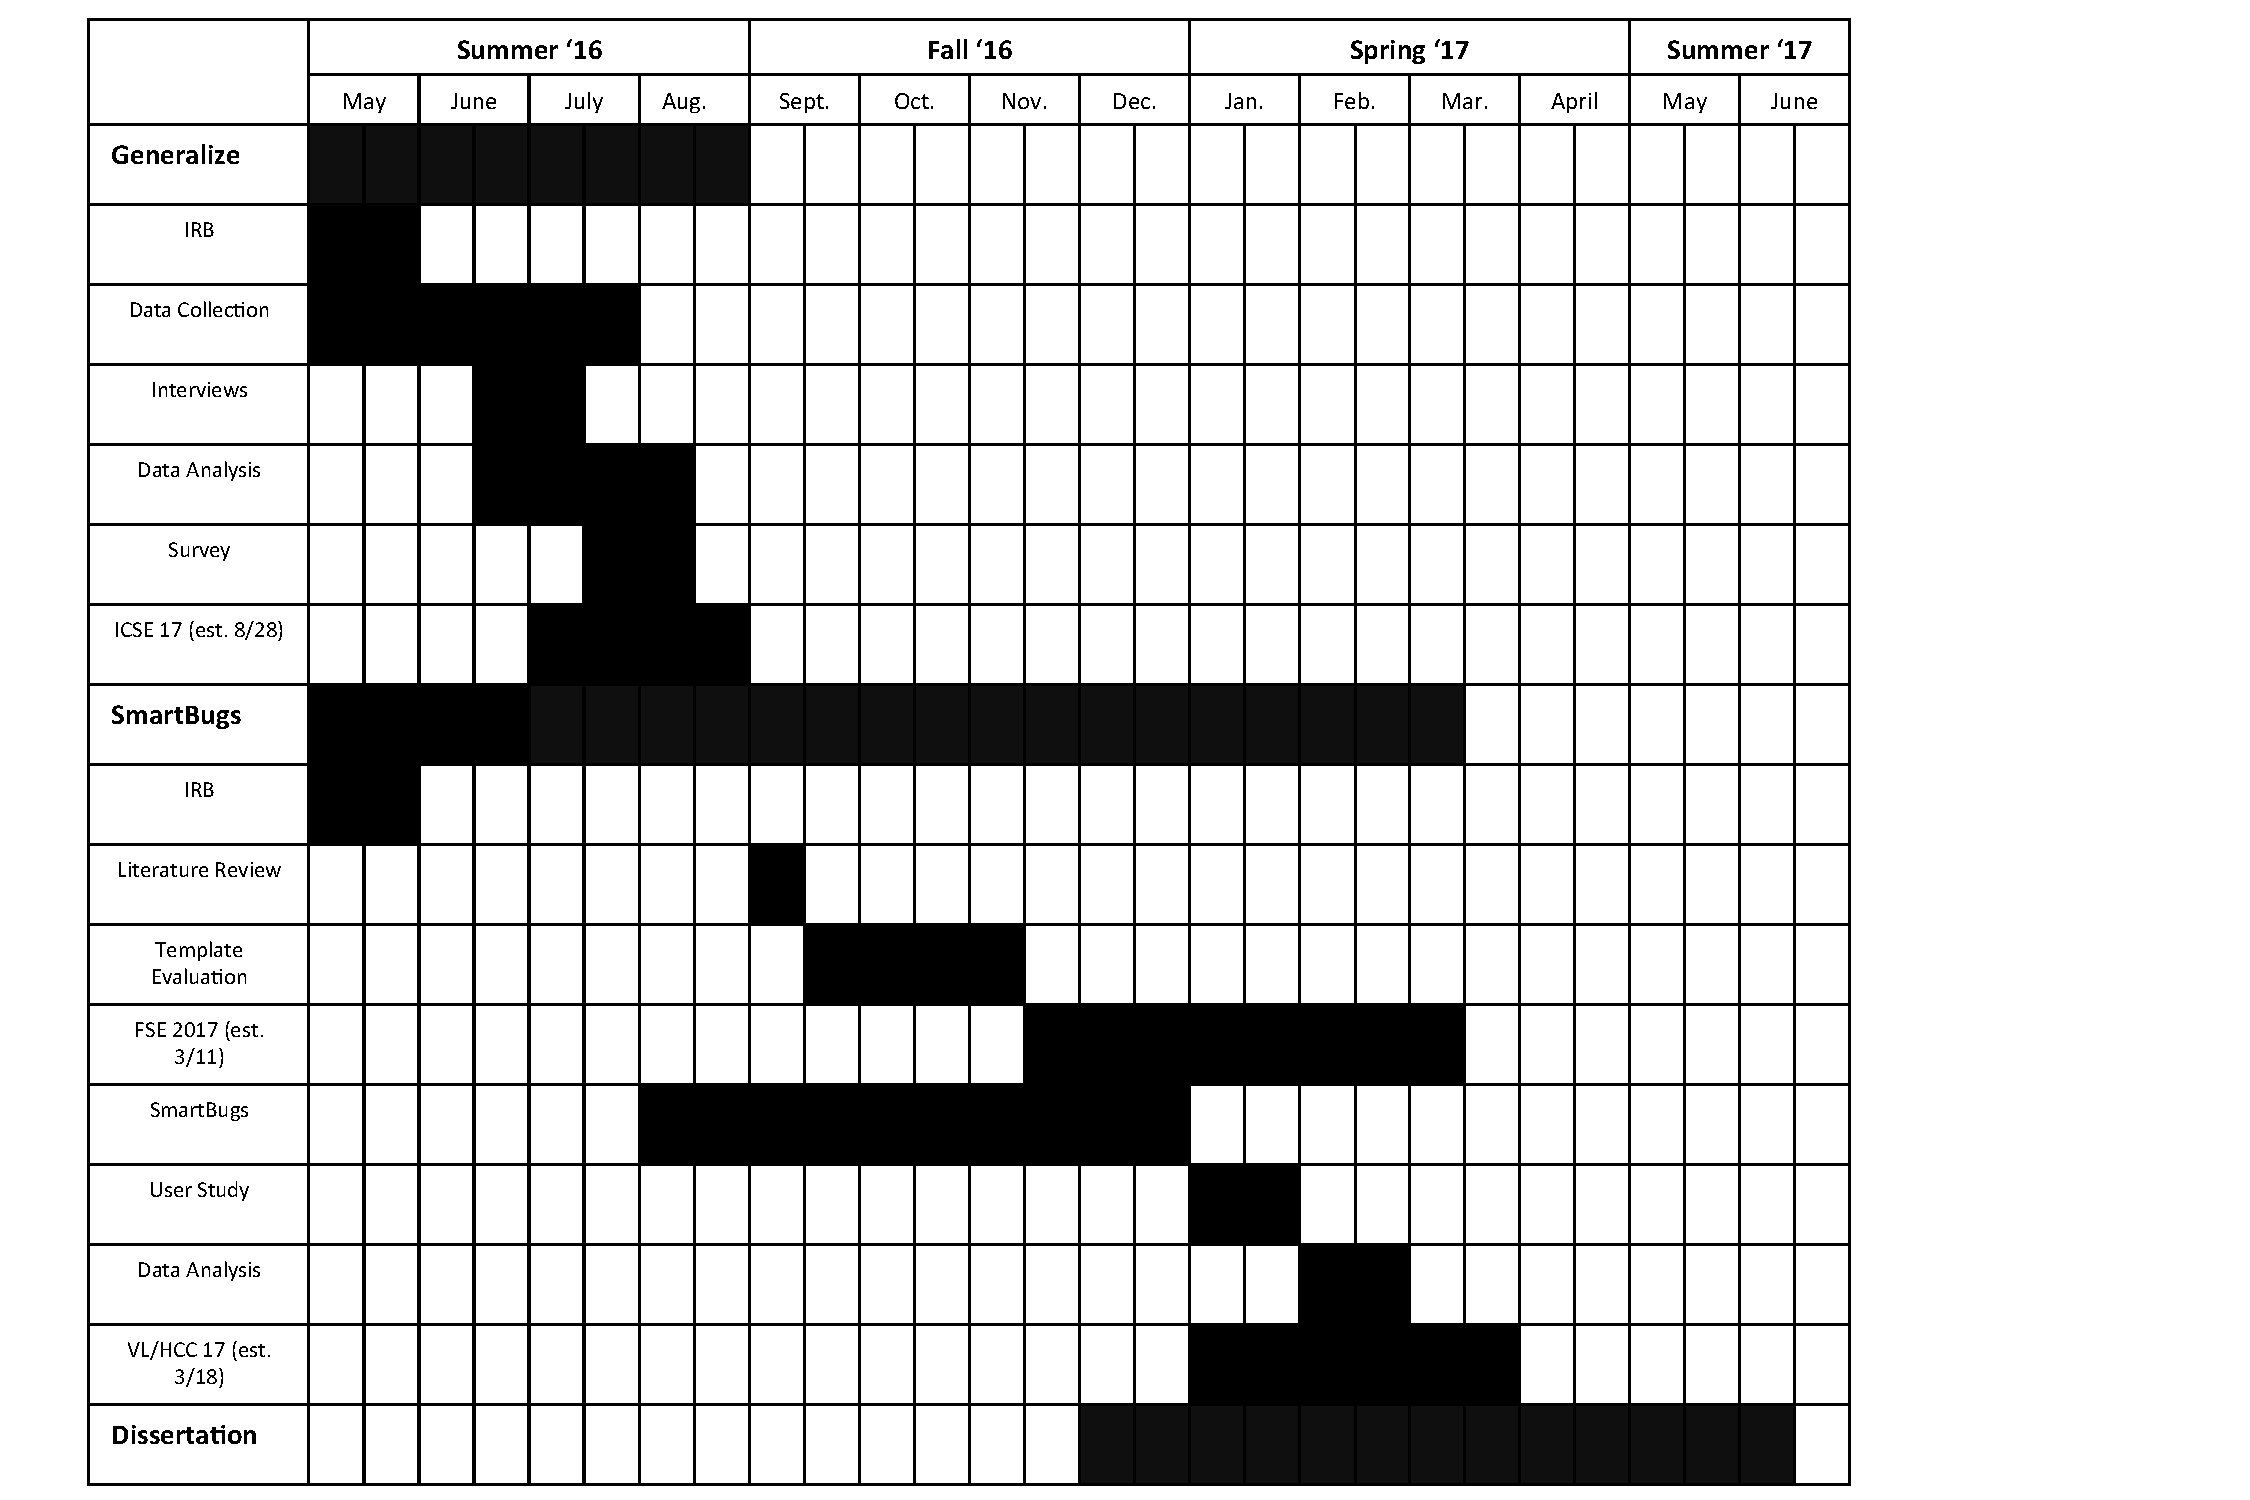
\includegraphics[width=5in]{figs/project-schedule.pdf}
	\caption{Month by month breakdown of plan to complete dissertation research.}
	\label{fig:plan}
\end{figure}

\subsection{Completed Projects \& Publications}

I have completed the following projects \& publications:
\begin{description}
	\item[Reasons] Completed Fall 2012; Publication: ICSE 2013
	\item[Challenges] Completed Fall 2015; Publication: FSE 2016 (in submission)
	\item[Predictions] Completed Spring 2016; Publication: VL/HCC 2016 (in submission)
\end{description}

\subsection{Upcoming Projects \& Publications}

I plan to complete the following projects \& publications by my defense in Spring 2017 (shown in Figure~\ref{fig:plan}):

\begin{description}
	\item[Generalize] (in progress) \textit{Amend IRB for interviews and survey} (May 1 -- June 1); \textit{Data collection} (May 3 -- July 31); \textit{Conduct Interviews} (June 15 -- July 15); \textit{Data analysis} (June 15 -- August 15) ; \textit{Survey and Analysis} (July 15 -- August 15); \textit{Publication}: ICSE 2017 (est. 8/28)
	\item[SmartBugs] \textit{Study IRB} (May 1 -- June 1); \textit{Literature Review} (September 1 -- September 15); \textit{Notification Template Evaluation} (September 15 - December 1); \textit{Publication}: FSE 2017 (est. 3/11); \textit{Develop SmartBugs} (with aide of Master's student) (August 1 -- January 1, 2017); \textit{User Study} (January 1 -- February 1 2017); \textit{Data analysis} (February 1 -- March 1); \textit{Write and edit draft} (January 1 - March 18); \textit{Publication}: VL/HCC 2017 (est. 3/18)
	% TODO SmartBugs study to VL/HCC and notifcation user eval to FSE?
	\item[Dissertation] \textit{Write and edit draft} (January 1 -- May 1) ; \textit{Publication}: Thesis Document
\end{description}

%ICSE 2017

%FSE2017

%VLHCC (backup?)

% JOURNAL??

\section*{Acknowledgments}
This material is based upon work supported by the National Science Foundation under
Grant No. 1217700, a Google Faculty Award, and a National Science Foundation
Graduate Research Fellowship under Grant No. DGE--0946818.
Special thanks to Emerson Murphy-Hill, Sarah Heckman, and the Developer Liberation Front, AltCode, and RealSearch research groups for their contributions and feedback.

\bibliographystyle{splncs03}
\bibliography{main.bib}

%
%\begin{thebibliography}{[MT1]}
%%
%\bibitem[CE1]{clar:eke}
%Clarke, F., Ekeland, I.:
%Nonlinear oscillations and
%boundary-value problems for Hamiltonian systems.
%Arch. Rat. Mech. Anal. 78, 315--333 (1982)
%%
%\bibitem[CE2]{clar:eke:2}
%Clarke, F., Ekeland, I.:
%Solutions p\'{e}riodiques, du
%p\'{e}riode donn\'{e}e, des \'{e}quations hamiltoniennes.
%Note CRAS Paris 287, 1013--1015 (1978)
%%
%\bibitem[MT1]{mich:tar}
%Michalek, R., Tarantello, G.:
%Subharmonic solutions with prescribed minimal
%period for nonautonomous Hamiltonian systems.
%J. Diff. Eq. 72, 28--55 (1988)
%%
%\bibitem[Ta1]{tar}
%Tarantello, G.:
%Subharmonic solutions for Hamiltonian
%systems via a $\bbbz_{p}$ pseudoindex theory.
%Annali di Matematica Pura (to appear)
%%
%\bibitem[Ra1]{rab}
%Rabinowitz, P.:
%On subharmonic solutions of a Hamiltonian system.
%Comm. Pure Appl. Math. 33, 609--633 (1980)
%\end{thebibliography}

%
\end{document}
